
%%% Local Variables:
%%% mode: latex
%%% TeX-master: t
%%% End:



\chapter{弹性波模式解耦全波形反演}
\label{cha:MD-EFWI}
\section{引言}
针对地下介质的定量成像方法对于刻画油气储层,监测CO$_2$注入以及估计近地表土壤和岩石的物理性
质非常有必要。相比于从地震偏移获得的定性化的叠后反射系数,我们更加希望得到定量化的深度域弹
性参数。地震反演旨在采用迭代的优化类方法通过拟合模拟数据与实际观测数据来恢复地下的真实模型。
不同于层析反演方法,例如Luo and Schuster (1991)\citep{luo1991},只采用走时信息,而全波形反演方法(FWI)提供
了更加完整的思路,同时采用走时与振幅信息来反演\cite[]{tarantola:1986}。
随着长偏移距、宽方位和宽频带采集的出现,全波形反演已经成为构建速度模型和进行定量地震成像的有效工具\cite{virieux2009overview}。

然而,FWI所需计算量十分巨大,尤其是在三维模型反演中。因此尽管梯度类的局部优化方法并不能保证反演收敛到全局最优解,
但是由于计算代价小其仍然被广泛应用与FWI中。而更能保证收敛的基于Hessian的求解方法\cite{mora:1987,crase1990robust}
由于更昂贵的计算代价则更多被FWI所舍弃。此外,为了减少计算量,我们通常采用声学近似来获得P波速度\cite{ravaut2004multiscale,operto2006crustal}。
但实际中,即使是以P波为主的无模式转换的单分量地震数据而言,声学近似也只能保证运动学信息的准确,振幅信息只有在小角度入射时才有保证。
这也是声波FWI通常需要非常仔细的数据预处理与预条件。总而言之,地震数据中总是包含弹性波的传播,即使在海上勘探中,
声波反演中并不能考虑到由于模式转换带来的能量损失,这就会对声波数据的产生过高拟合从而低估模型中界面反差。

弹性波全波形反演(EFWI)\cite{tarantola:1986}能够从多分量数据中反演地下介质的弹性参数,如P/S-波速度和密度。
尽管其仍然需要很大计算代价,EFWI还是在很多实际数据中获得了应用
\cite{crase1992nonlinear,djikpesse.tarantola:1999,sears2008,sears:2010,prieux:2013a,prieux:2013b,vigh:2014}。
EFWI的实现方式可以在时间域\cite{shipp:2002},可以在频率域\cite{brossier2009},也可以采用混合的方式在时间域进行正演模拟而在频率域求解
\cite{nihei.li:2007,sirgue:2008}。然而,EFWI中多个参数参与反演会增加反问题的非线性程度,同时也会受到由于不同物理参数之间的串扰带来的反演
中参数耦合的影响\cite{forgues.lambare:1997}。在海洋环境中,尤其是在软海底环境中,由于P-to-
S的转换模式非常弱,基于拖缆或者海底多分量数据的EFWI的非线性程度会变得更严重\cite{sears2008}。

很多学者指出参数化方式对缓解参数耦合效应非常重要,通常可以通过调查散射模式或者Hessian算子来选取不同的参数化方式
\cite[]{wu.aki:1985,tarantola:1986,plessix.cao:2011,gholami2013}。另外一个常用的降低非线性程度的方法是采用多尺度的策略
将速度扰动分解为低波数与高波数成分\cite[]{symes.carazzone:1991,bunks1995multiscale,clement:2001,shin.cha:2008,dehoop:2012,
xu:2012,biondi.almomin:2013,ma.hale:2013,warner2016adaptive,alkhalifah2015scattering}。
将声波FWI扩展到弹性介质中学要付出更多的工作。正如Tarantola(1986)\cite{tarantola:1986}所建议的,我们应当先重构出对数据具有主要影响
的参数,然后再重构出对数据有次级影响的参数。Sears(2008)\cite{sears2008}提出了一个有效的多尺度策略,通过时间窗来选取海底电缆(OBC)
数据中的不同子集来进行多尺度反演。Operto(2013)\cite{operto2013guided}讨论了如何多级地选取不同的数据分量以及不同的参数类型进行反演,从而
控制参数之间的耦合效应并降低反演的非线性。Xu和mcmechan\cite{xu.mcmechan:2014}提出了一个多步长的策略来提高密度模型的反演精度。

一个解决参数耦合行之有效的方法就是反演中考虑Hessian算子。Hessian逆的对角块能够消除几何扩散以及带限效应带来的模糊性,而非对角块能够压制
参数之间的耦合效应\cite[]{pratt1998gauss,fichtner2011hessian,operto2013guided,innanen2014seismic,pan2015estimation}。
为了避免不可承受的Hessian计算和求逆,很多研究工作都旨在找到对Hessian逆的有效近似,例如采用拟Hessian\cite[]{shin2001improved,choi.shin:2008}
或者通过拟牛顿方式迭代构建Hessian核函数,如L-BFGS方法\cite[]{nocedal2006numerical,brossier2009}。
Sheen et al(2006)\cite{sheen:2006}通过互易原理和褶积定理来计算近似Hessian从而实现了时间域的Gauss-Newton (GN) EFWI方法。
Bae et al(2012)\cite{bae:2012}提出了频率域基于GN共轭梯度法的声弹耦合FWI。
Pratt et al(1998)\cite{pratt1998gauss}采用“虚震源”引起的偏导数波场的概念解释了梯度与Hessian算子的物理含义。参数耦合效应是由于
不同参数的偏导数波场在特定角度范围内的重叠导致的。因此,Wang et al\cite{wang:2015}在EFWI中,通过解耦弹性波波场并在不同阶段分别选取P波与S波
数据来反演不同参数从而压制参数耦合。通过调查解耦之后的P波与S波目标函数,Ren and Liu\cite{ren.liu:2016}证明了波场的解耦可以降低EFWI的非线性程度。
此外,模式解耦也是弹性波逆时偏移中获得具有物理含义成像的关键步骤\cite{yan:2008,wang2016scalar}。

在本文中,我们并未经验性的通过解耦正、反传波场以及地震记录\cite{ren.liu:2016},而是采用了更有物理意义同时更节省计算量的预条件方式,
也即只解耦反传波场。为了简单起见,我们不在正文中考虑密度反演,而是在讨论部分进行部分阐述。首先,通过弹性波Born近似,我们分析了P波速度与S波速度扰动的
辐射模式,并导出了解耦的Frech{$\acute{e}$}t导数或Jacobian矩阵;然后,我们调查了解耦后的P波与S波数据对梯度的贡献并提出了在梯度计算中的交叉项近似。
在此基础上,预条件的梯度可以通过伴随状态法\cite[]{plessix2006}快速有效地计算得到,也即正传波场与解耦后反传波场的零延迟互相关。
然后,为了获得更多物理机制上的认识,我们计算并分析了基于解耦的Hessian和分辨率矩阵,同时也比较了MD预条件后的梯度与GN梯度的异同。
此后,我们通过在流体饱和沙岩模型以及Marmousi-II模型的数值实验证明了基于解耦的EFWI的有效性。
最后,我们给出关于密度反演的简单讨论并获得了一些结论。

\section{弹性波正问题}
\label{sec:forward_problem}
地球的地下模型可以被认为是弹性假设下的弹性介质。地震波波场在弹性介质中传播的控制方程可以写作:
\begin{equation}
	\rho \frac{\partial u^2_i}{\partial t^2}  -
	\frac{\partial}{\partial x_j}\left[c_{ijkl}\frac{\partial u_{k}}{\partial
	x_l}\right]=f_i,
	\label{eq:WE} 
\end{equation}
其中$u_i$和$f_i$ 分别为质点位移矢量的第$i$分量以及震源项,$\rho$为密度,$c_{ijkl}$
为刚度矩阵张量的分量。上述所有的下标取值为从1到3,并且重复下标的Einstein求和方式被默认隐含在其中。
对于各向同性介质而言,刚度矩阵张量满足:
\begin{equation}
	c_{ijkl}=\lambda\delta_{ij}\delta
	_{kl}+\mu(\delta_{ik}\delta _{jl}+\delta _{il}\delta_{jk}),
	\label{Lame}
\end{equation}
其中,$\lambda$和$\mu$为Lam$\acute{e}$系数,$\delta_{ij}$为Kronecker函数。 

根据Born近似,在$\mathbf{x}$ 位置上对刚度系数做一个微小扰动,$\delta
c_{ijkl}(\mathbf{x})$,将会产生一个扰动波场:
\begin{equation}
	\rho \frac{\partial \delta u^2_i}{\partial t^2}  -
	\frac{\partial}{\partial x_j}\left[c^0_{ijkl}\frac{\partial \delta u_{k}}{\partial
	x_l}\right]=\frac{\partial}{\partial
	x_j}\left[\delta c_{ijkl}\frac{\partial
	u^0_{k}}{\partial x_l}\right]. 
	\label{eq:BornApp}
\end{equation}
其中,$\mathbf{u}^0$为在背景介质$c^0_{ijkl}$中满足方程\eqref{eq:WE}
的背景场。上式说明扰动场可看作是入射波场与参数扰动$\delta
c_{ijkl}(\mathbf{x})$相互作用产生的次级源所引发。为了简单起见,本章的公式推导主要在频率域进行,但是大部分的计算操作则在时间域实现。
利用表示定理与散度定理(Kamath and Tsvankin, 2016)\cite{kamath2016elastic},扰动波场满足:
\begin{equation}
	\delta u_n(\mathbf{r},\omega)=-\int_{\Omega(\mathbf{x})}{\frac{\partial
	u^0_{k}(\mathbf{x},\omega)}{\partial x_l}
	\frac{\partial G_{ni}(\mathbf{r},\mathbf{x},\omega)}{\partial
	x_j} \delta
	c_{ijkl}(\mathbf{x})}
	d\Omega(\mathbf{x}), \quad (n=1,2,3),
	\label{eq:Repre}
\end{equation}
其中,$\omega$表示频率,$G_{ni}(\mathbf{r},\mathbf{x},\omega)$为弹性波背景格林函数,表示在$\mathbf{x}$处沿$i$方向的单位体力源
所产生的在$\mathbf{r}$处沿$n$方向的质点位移,$\Omega(\mathbf{x})$为体积积分范围。注意方程\eqref{eq:Repre}只考虑了一阶散射的情况。
刚度系数扰动与速度扰动之间的关系为:
\begin{equation}
        \delta c_{ijkl}=\frac{\partial c_{ijkl}}{\partial V_p}\delta V_p
        +\frac{\partial c_{ijkl}}{\partial V_s}\delta V_s,
        \label{eq:deltaLame}
\end{equation}
以及
\begin{equation}
        \begin{split}
                &\frac{\partial c_{ijkl}}{\partial V_p}=2\rho V_p\delta_{ij}\delta_{kl},\\
                &\frac{\partial c_{ijkl}}{\partial V_s}=2\rho
                V_s(-2\delta_{ij}\delta_{kl}+\delta_{ik}\delta _{jl}+\delta_{il}\delta_{jk}),
        \end{split}
        \label{eq:deltaLame}
\end{equation}
将方程\eqref{eq:Repre}重写为速度参数化方式:
\begin{equation}
        \delta
        u_n(\mathbf{r},\omega)=\int_{\Omega(\mathbf{x})}{\left[J_{n,V_p}(\mathbf{r,x},\omega)\delta
                V_p(\mathbf{x}) +J_{n,V_s}(\mathbf{r,x},\omega)\delta
        V_s(\mathbf{x})\right]
                }
                d\Omega(\mathbf{x}),
        \label{eq:SplitRepre}
\end{equation}
其中
\begin{equation}
        J_{n,M}(\mathbf{r,x},\omega)=
        T_{ij,M}(\mathbf{x},\omega)G_{ni,j}(\mathbf{r,x},\omega), \quad M\in\{V_p,V_s\},
\label{eq:KernelAB}
\end{equation}
并且
\begin{equation}
\begin{split}
                &T_{ij,M}(\mathbf{x},\omega)=\frac{\partial c_{ijkl}}{\partial M}\frac{\partial
                        u^0_{k}(\mathbf{x},\omega)}{\partial x_l},\\ 
                        &G_{ni,j}(\mathbf{r,x},\omega)=\frac{\partial
                                G_{ni}(\mathbf{r},\mathbf{x},\omega)}{\partial x_j},
\end{split}
\label{eq:traction}
\end{equation}
上述中$J_{n,M}$表示速度扰动对应的偏导数波场\cite[]{pratt1998gauss},$T_{ij,M}$
表示背景波场$u^0$与速度扰动$\delta V_p$ (或 $\delta V_s$)
作用产生的次级震源,$G_{ni,j}$表示格林函数的空间导数。假设模型网格数与接收点个数为L和K,则方程\eqref{eq:KernelAB}可以重写为离散的形式:
\begin{equation}
        \mathbf{J}_{n,M}(\mathbf{x}_l,\mathbf{r}_k)=
        (\mathbf{T}_M(\mathbf{x}_l):\mathbf{G}'(\mathbf{x}_l,\mathbf{r}_k))_n,\quad
        k=1,2,...,K;\quad l=1, 2,...,L,
        \label{eq:EquivFre}
\end{equation}
其中的双点符号$:$代表了以下操作:
\begin{equation}
    (\mathbf{T}_M:\mathbf{G}')_{n}=\sum_{i,j=1}^{3}T_{ij,M}G_{ni,j}.
    \label{eq:contraction}
\end{equation}
这里为了简化表达我们隐藏了下标$n$来代表多分量数据。因此,方程\eqref{eq:SplitRepre}可写成矩阵形式:
\begin{equation}
            \begin{pmatrix}
                        \mathbf{J}_{V_p}&\quad\mathbf{J}_{V_s}
    \end{pmatrix}
    \begin{pmatrix}
       \delta  \mathbf{V}_p\\
       \delta \mathbf{V}_s
    \end{pmatrix}
    =
        \mathbf{\delta u},
        \label{eq:finalMatrix}
\end{equation}
其中$\mathbf{J}_{V_p}$和$\mathbf{J}_{V_s}$为$K\times L$大小的Frech{$\acute{e}$}t导数(Jacobian矩阵),
$\delta \mathbf{V}_p$和$\delta \mathbf{V}_s$为长度为$L$的模型参数向量,$\delta \mathbf{u}$为在接收点位置上的弹性散射波场。
则方程\eqref{eq:finalMatrix}可以简化为:
\begin{equation}
        \mathbf{J}\delta \mathbf{m}
    =
        \mathbf{\delta u},
        \label{eq:finalMatrixshort}
\end{equation}
with $\mathbf{J}=(\mathbf{J}_{V_p}\quad\mathbf{J}_{V_s})$ and
$\delta \mathbf{m}=(\delta\mathbf{V}_p \quad \delta\mathbf{V}_s)^T$.

方程\eqref{eq:finalMatrix}或\eqref{eq:finalMatrixshort}说明Jacobian矩阵与参数扰动向量的乘积即为相应的散射数据响应,而所有该数据响应的
叠加就组成了整个散射波波场。从图\ref{fig:radiationpattern}中展示的散射模式可看出,$\delta V_p$只通过PP模式散射P波数据,而$\delta V_s$
则散射所有模式的P波和S波数据。因此这就很难分辨出散射数据中的P波是来自于哪一类速度扰动($\delta V_p$或$\delta V_s$)。
幸运的是,散射S波则仅仅由$V_s$产生,因而对于单次散射的弹性波数据来讲,耦合效应只会出现在P波的模式中。
反演中的参数耦合效应是由于不同模型参数的偏导数波场在特定角度范围内的重叠导致的\cite{tarantola:1986,operto2013guided}。
所以很自然地,我们采用模式解耦来作为EFWI中降低参数耦合效应的工具。
\begin{figure}[!htb]
    \begin{center}
        \subfloat[]{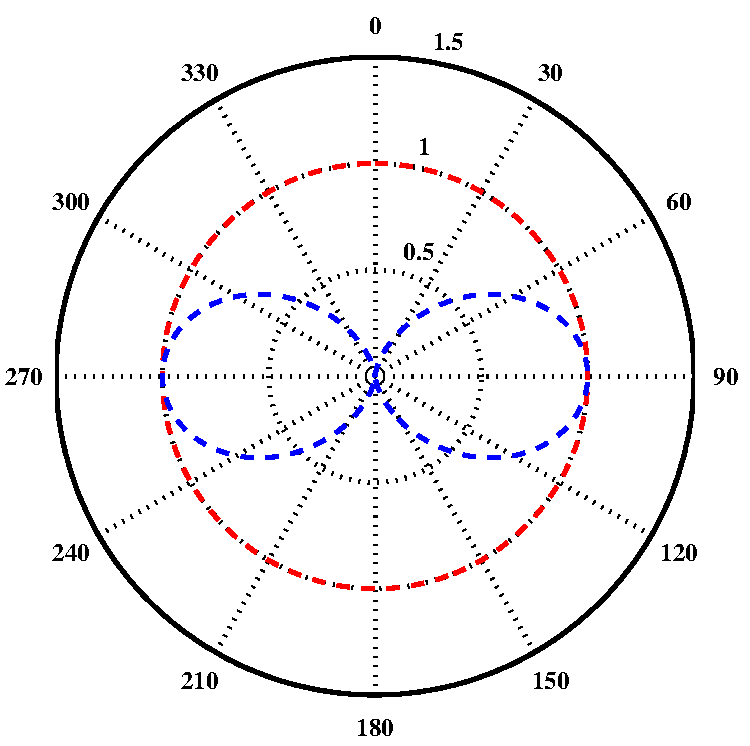
\includegraphics[width=5cm]{Figure/chapter02/radiationpattern/Fig/PP.pdf}}
%        \subfloat{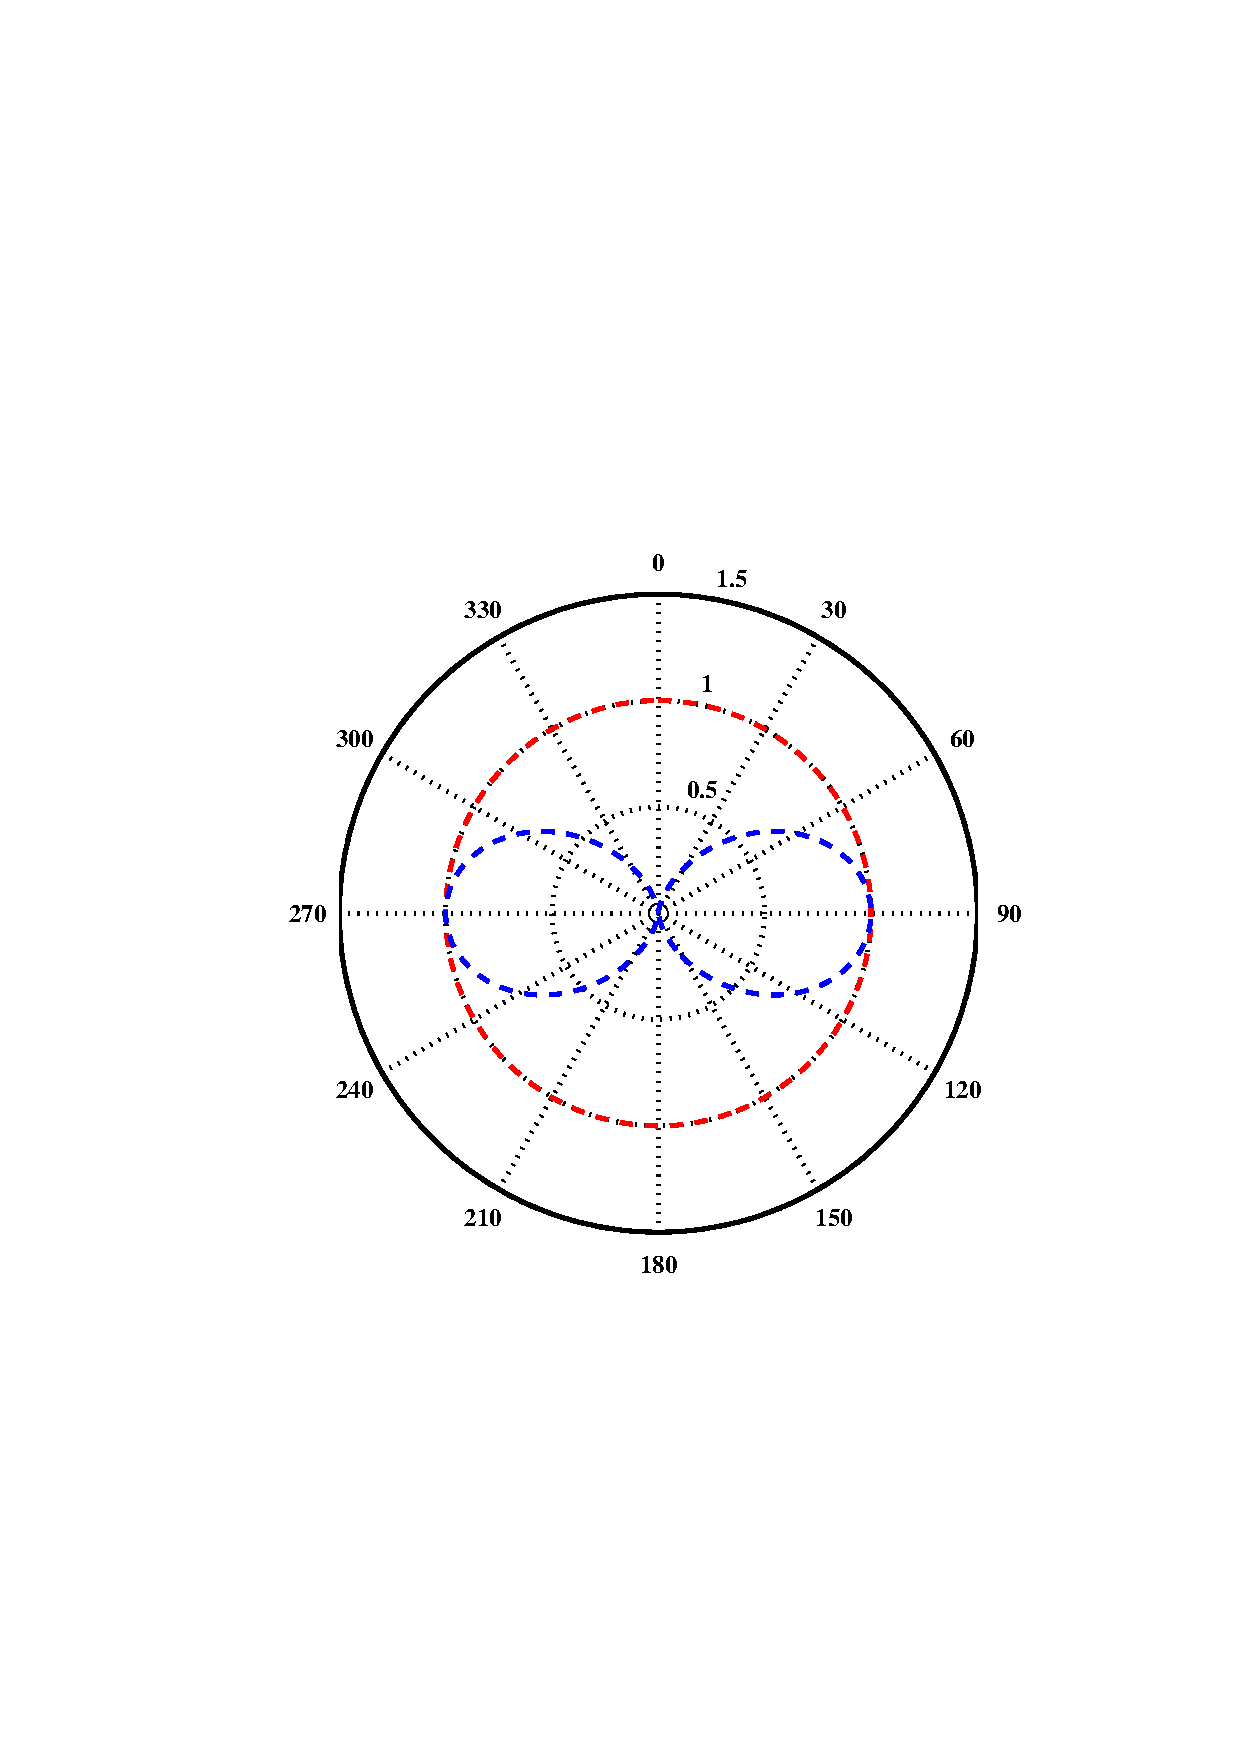
\includegraphics[width=5cm]{radiationpattern/Fig/PP.pdf}}
        \subfloat[]{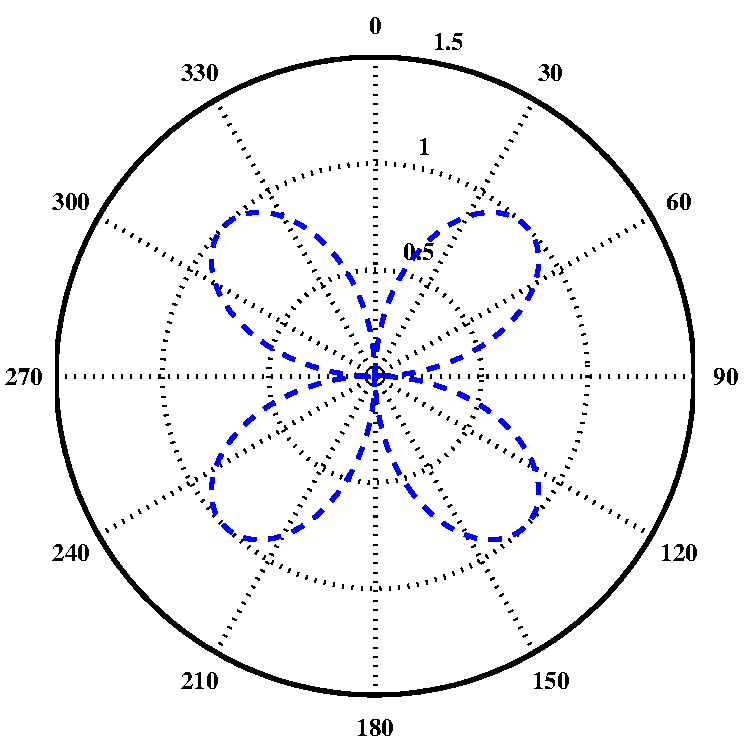
\includegraphics[width=5cm]{Figure/chapter02/radiationpattern/Fig/PS.pdf}}\\
        \subfloat[]{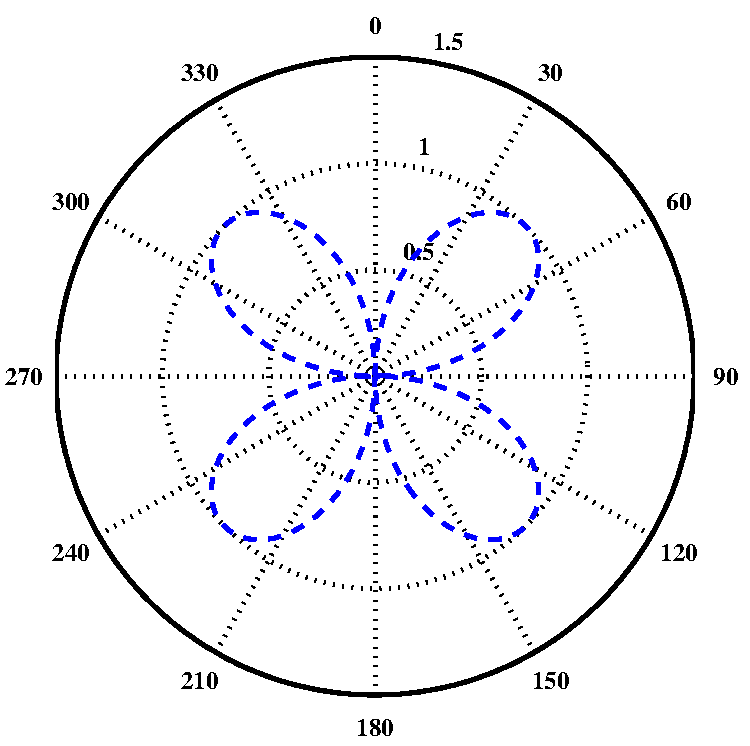
\includegraphics[width=5cm]{Figure/chapter02/radiationpattern/Fig/SP.pdf}}
        \subfloat[]{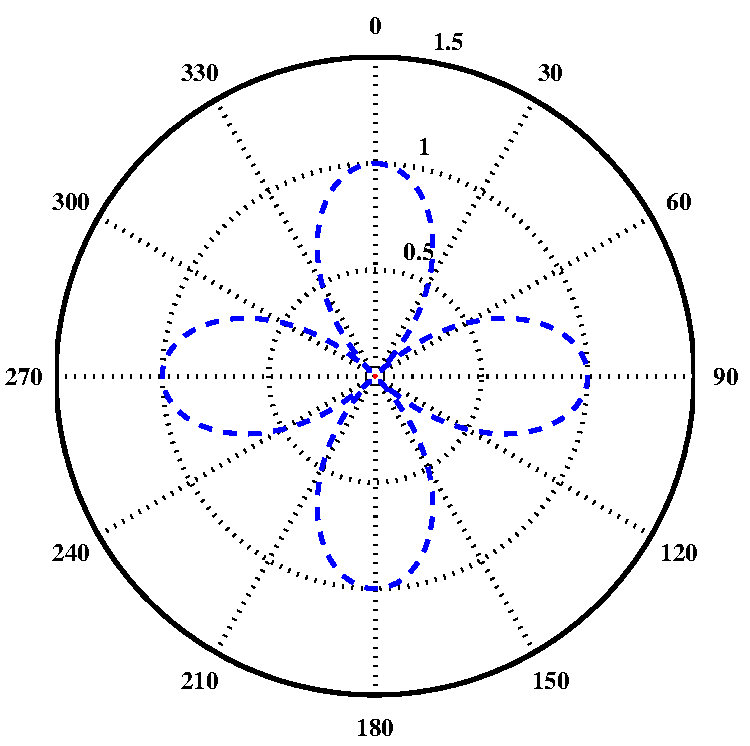
\includegraphics[width=5cm]{Figure/chapter02/radiationpattern/Fig/SS.pdf}}
        \caption{$V_p$(red)和$V_s$ (blue)扰动的辐射模式 . (a) PP, (b) PS, (c) SP and (d) SS模式.
    }
    \label{fig:radiationpattern} 
    \end{center}
\end{figure} 

\subsection{弹性波模式解耦}
弹性波波场$\mathbf{u}=(u_x,u_y,u_z)$可以分解成P波波场与S波波场:$\mathbf{u}=\mathbf{u}^P+\mathbf{u}^S$,
其中,$\mathbf{u}^P=(u^P_x,u^P_y,u^P_z)$和$\mathbf{u}^S=(u^S_x,u^S_y,u^S_z)$.
对于各向同性介质而言,该模式解耦方式是不依赖于模型参数的,可在波数域表征为(Zhang and McMechan, 2010)\cite[]{zhang.mcmechan:2010}:
\begin{equation}
        \tilde{\mathbf U}^P=\mathbf k(\mathbf k\cdot \tilde{\mathbf U}), \quad
        \tilde{\mathbf U}^S=-\mathbf 
        k\times(\mathbf k\times \tilde{\mathbf U})
\label{eq:Decomp}
\end{equation}
其中$\mathbf k=(k_x,k_y,k_z)$ 为归一化之后的波矢量,符号$\tilde{}$表示波数域波场。

根据以上推导, 我们将Fr{$\acute{e}$}chet导数分解为不同波模式:
\begin{equation}
        {\mathbf J}_M={\mathbf J}^P_M+{\mathbf J}^S_M,
\label{eq:PropaMDall}
\end{equation}
其中
\begin{equation}
        {\mathbf J}^P_M=\mathcal{F}^{-1}(\mathbf k(\mathbf k\cdot \tilde{\mathbf
        J}_M)), \quad
        {\mathbf J}^S_M=\mathcal{F}^{-1}(-\mathbf
                k\times(\mathbf k\times \tilde{\mathbf J}_M)),
\label{eq:PropaMDsplit}
\end{equation}
其中$\mathcal{F}^{-1}$表示从波数域到空间域的反Fourier变换,$\tilde{\mathbf{J}}_M$表示波数域的 Frech{$\acute{e}$}t导数。
这样,方程\eqref{eq:finalMatrixshort}可以按以下方式分裂成两部分:
\begin{equation}
        \mathbf{J}^P\delta\mathbf{m}=\mathbf{\delta u}^P,\quad
        \mathbf{J}^S\delta\mathbf{m}=\mathbf{\delta u}^S,
        \label{eq:UPandUS}
\end{equation}
其中
\begin{equation}
        \mathbf{\delta u}=\mathbf{\delta u}^P+\mathbf{\delta u}^S,
        \label{eq:UPS}
\end{equation}
并且
\begin{equation}
        \mathbf{J}=\mathbf{J}^P+\mathbf{J}^S,
        \label{eq:JPS}
\end{equation}
其中$\mathbf{J}^P=(\mathbf{J}^P_{V_p}\quad\mathbf{J}^P_{V_s})$和$\mathbf{J}^S=(\mathbf{J}^S_{V_p}\quad\mathbf{J}^S_{V_s})$为大小是$K\times{2L}$的矩阵,分别代表P波或S波分量对应的Frech{$\acute{e}$}t导数(Jacobian矩阵)。
方程\eqref{eq:UPandUS}表示了在模式解耦下的Born近似所描述的散射波场。

注意到,次级震源只有在背景波场入射到参数扰动的位置时才会被激发。尽管次级震源(或者说背景场)中会既有P波又有S波,
但是我们发现对于反演来说并不需要严格区分出他们的贡献(原因我们将在讨论部分进行详细阐述)。因此,模式解耦下Jacobian
矩阵满足:
\begin{equation}
        \begin{split} 
        \mathbf{J}^W_M(\mathbf{x}_l,\mathbf{r}_k)=
        \mathbf{T}_M(\mathbf{x}_l):\mathbf{G}'^W(\mathbf{x}_l,\mathbf{r}_k),\quad
        W\in\{P, S\}.
        \end{split}
        \label{eq:EquivFre1}
\end{equation}
该式说明模式解耦算子只作用在了$\mathbf{G}'$上,也即散射Green函数的空间导数。虽然有些学者尝试用“解耦”的方式来
传播P和S波波场(马德堂和朱光明,2003\cite{马德堂2003}; Cheng et al.,
2016\cite{cheng:2016}),
但是他们只能在介质参数足够光滑的时候才能获得令人满意的结果(Brytik et al., 2011\cite{brytik:2011};
Wang and McMechan, 2015\cite{wang.mcmechan:2015b})。
因此,我们并未采用传播解耦波场的方法而是采用传播之后用方程\eqref{eq:PropaMDsplit}来进行模式解耦。

\section{弹性波模式解耦全波形反演}
方程\eqref{eq:finalMatrixshort}对应的反问题是要找到一个能够解释地震数据的最优模型。该问题的解可以通过求解以下
目标函数的最小值来获得:
\begin{equation}
    E=\frac{1}{2}\delta\mathbf{d}^{\dagger}\delta\mathbf{d},
    \label{eq:misfit}
\end{equation}
其中$\delta\mathbf{d}$ 表示观测数据与模拟数据之间的残差向量,满足$\delta\mathbf{d}=\mathfrak{F}(\mathbf{u}_{obs}-\mathbf{u}_{cal})$,
这里$\mathfrak{F}$ 为位于接收点处的重采样函数,上标$\dagger$表示共轭转置算子。求解该目标函数最小值的标准策略是
采用梯度类或者基于Hessian矩阵的最优化算法。可以通过Jacobian矩阵来求取梯度:
\begin{equation}
        \mathbf{g}=
        \begin{pmatrix}
                \mathbf{g}_{V_p}\\
                \mathbf{g}_{V_s}
        \end{pmatrix}
        =\mathfrak{R}\begin{pmatrix}
                \mathbf{J}^{\dagger}_{V_p}\delta \mathbf{d}\\
                \mathbf{J}^{\dagger}_{V_s}\delta \mathbf{d}
        \end{pmatrix},
        \label{eq:MatrixGra1}
\end{equation}
其中$\mathfrak{R}$表示只取结果的实部。为获得模型更新,梯度导引类方法利用$\mathbf{g}$,而Hessian类方法则利用了
梯度和Hessian矩阵的信息。Hessian类算法能保证四阶的收敛性但即使是声波FWI也要花费庞大的计算与存储代价。
为了在效率与精度之间寻求平衡,我们通常会采用梯度类的方法迭代地求解方程\eqref{eq:misfit},也即:
\begin{equation}
        \mathbf{m}_{k+1}=\mathbf{m}_{k}-\alpha_k \mathbf{g}_k,
        \label{eq:Gradientmethod}
\end{equation}
其中$\mathbf{m}$是模型参数向量,$k$是迭代次数,$\alpha_k$和$\mathbf{g}_k$则分别是第$k$迭代的步长与梯度。
常规的EFWI需要非常多的迭代次数,因此良好的梯度预条件能够加速收敛。

方程\eqref{eq:MatrixGra1}中的梯度并没有内在的机制来判断数据残差的中的变化是来自$\delta V_p$还是来自$\delta V_s$。
我们将方程\eqref{eq:MatrixGra1}分裂为P波与S波分量对应的两个部分:
\begin{equation}
        \begin{pmatrix}
                \mathbf{g}^P_{V_p}\\
                \mathbf{g}^P_{V_s}
        \end{pmatrix}
        =\mathfrak{R}\begin{pmatrix}
                [\mathbf{J}^P_{V_p}+\mathbf{J}^S_{V_p}]^{\dagger}\delta \mathbf{d}^P\\
                [\mathbf{J}^P_{V_s}+\mathbf{J}^S_{V_s}]^{\dagger}\delta \mathbf{d}^P
        \end{pmatrix},
        \label{eq:DEMatrixGraP}
\end{equation}
和
\begin{equation}
        \begin{pmatrix}
                \mathbf{g}^S_{V_p}\\
                \mathbf{g}^S_{V_s}
        \end{pmatrix}
        =\mathfrak{R}\begin{pmatrix}
                [\mathbf{J}^P_{V_p}+\mathbf{J}^S_{V_p}]^{\dagger}\delta \mathbf{d}^S\\
                [\mathbf{J}^P_{V_s}+\mathbf{J}^S_{V_s}]^{\dagger}\delta \mathbf{d}^S
        \end{pmatrix},
        \label{eq:DEMatrixGraS}
\end{equation}
其中,$\mathbf{g}^W_M$为特定波模式(W)的数据残差对应的某一物理参数(M)的梯度。
由于在地面进行P/S数据的分离非常具有挑战,因此数据残差的的分解也会变得非常困难,尤其是在近地表介质非均匀且(或者)
边界条件不完整的情况下。因此需要采取策略来回避多分量地震记录的地面分解。
\begin{figure*}
    \begin{center}
        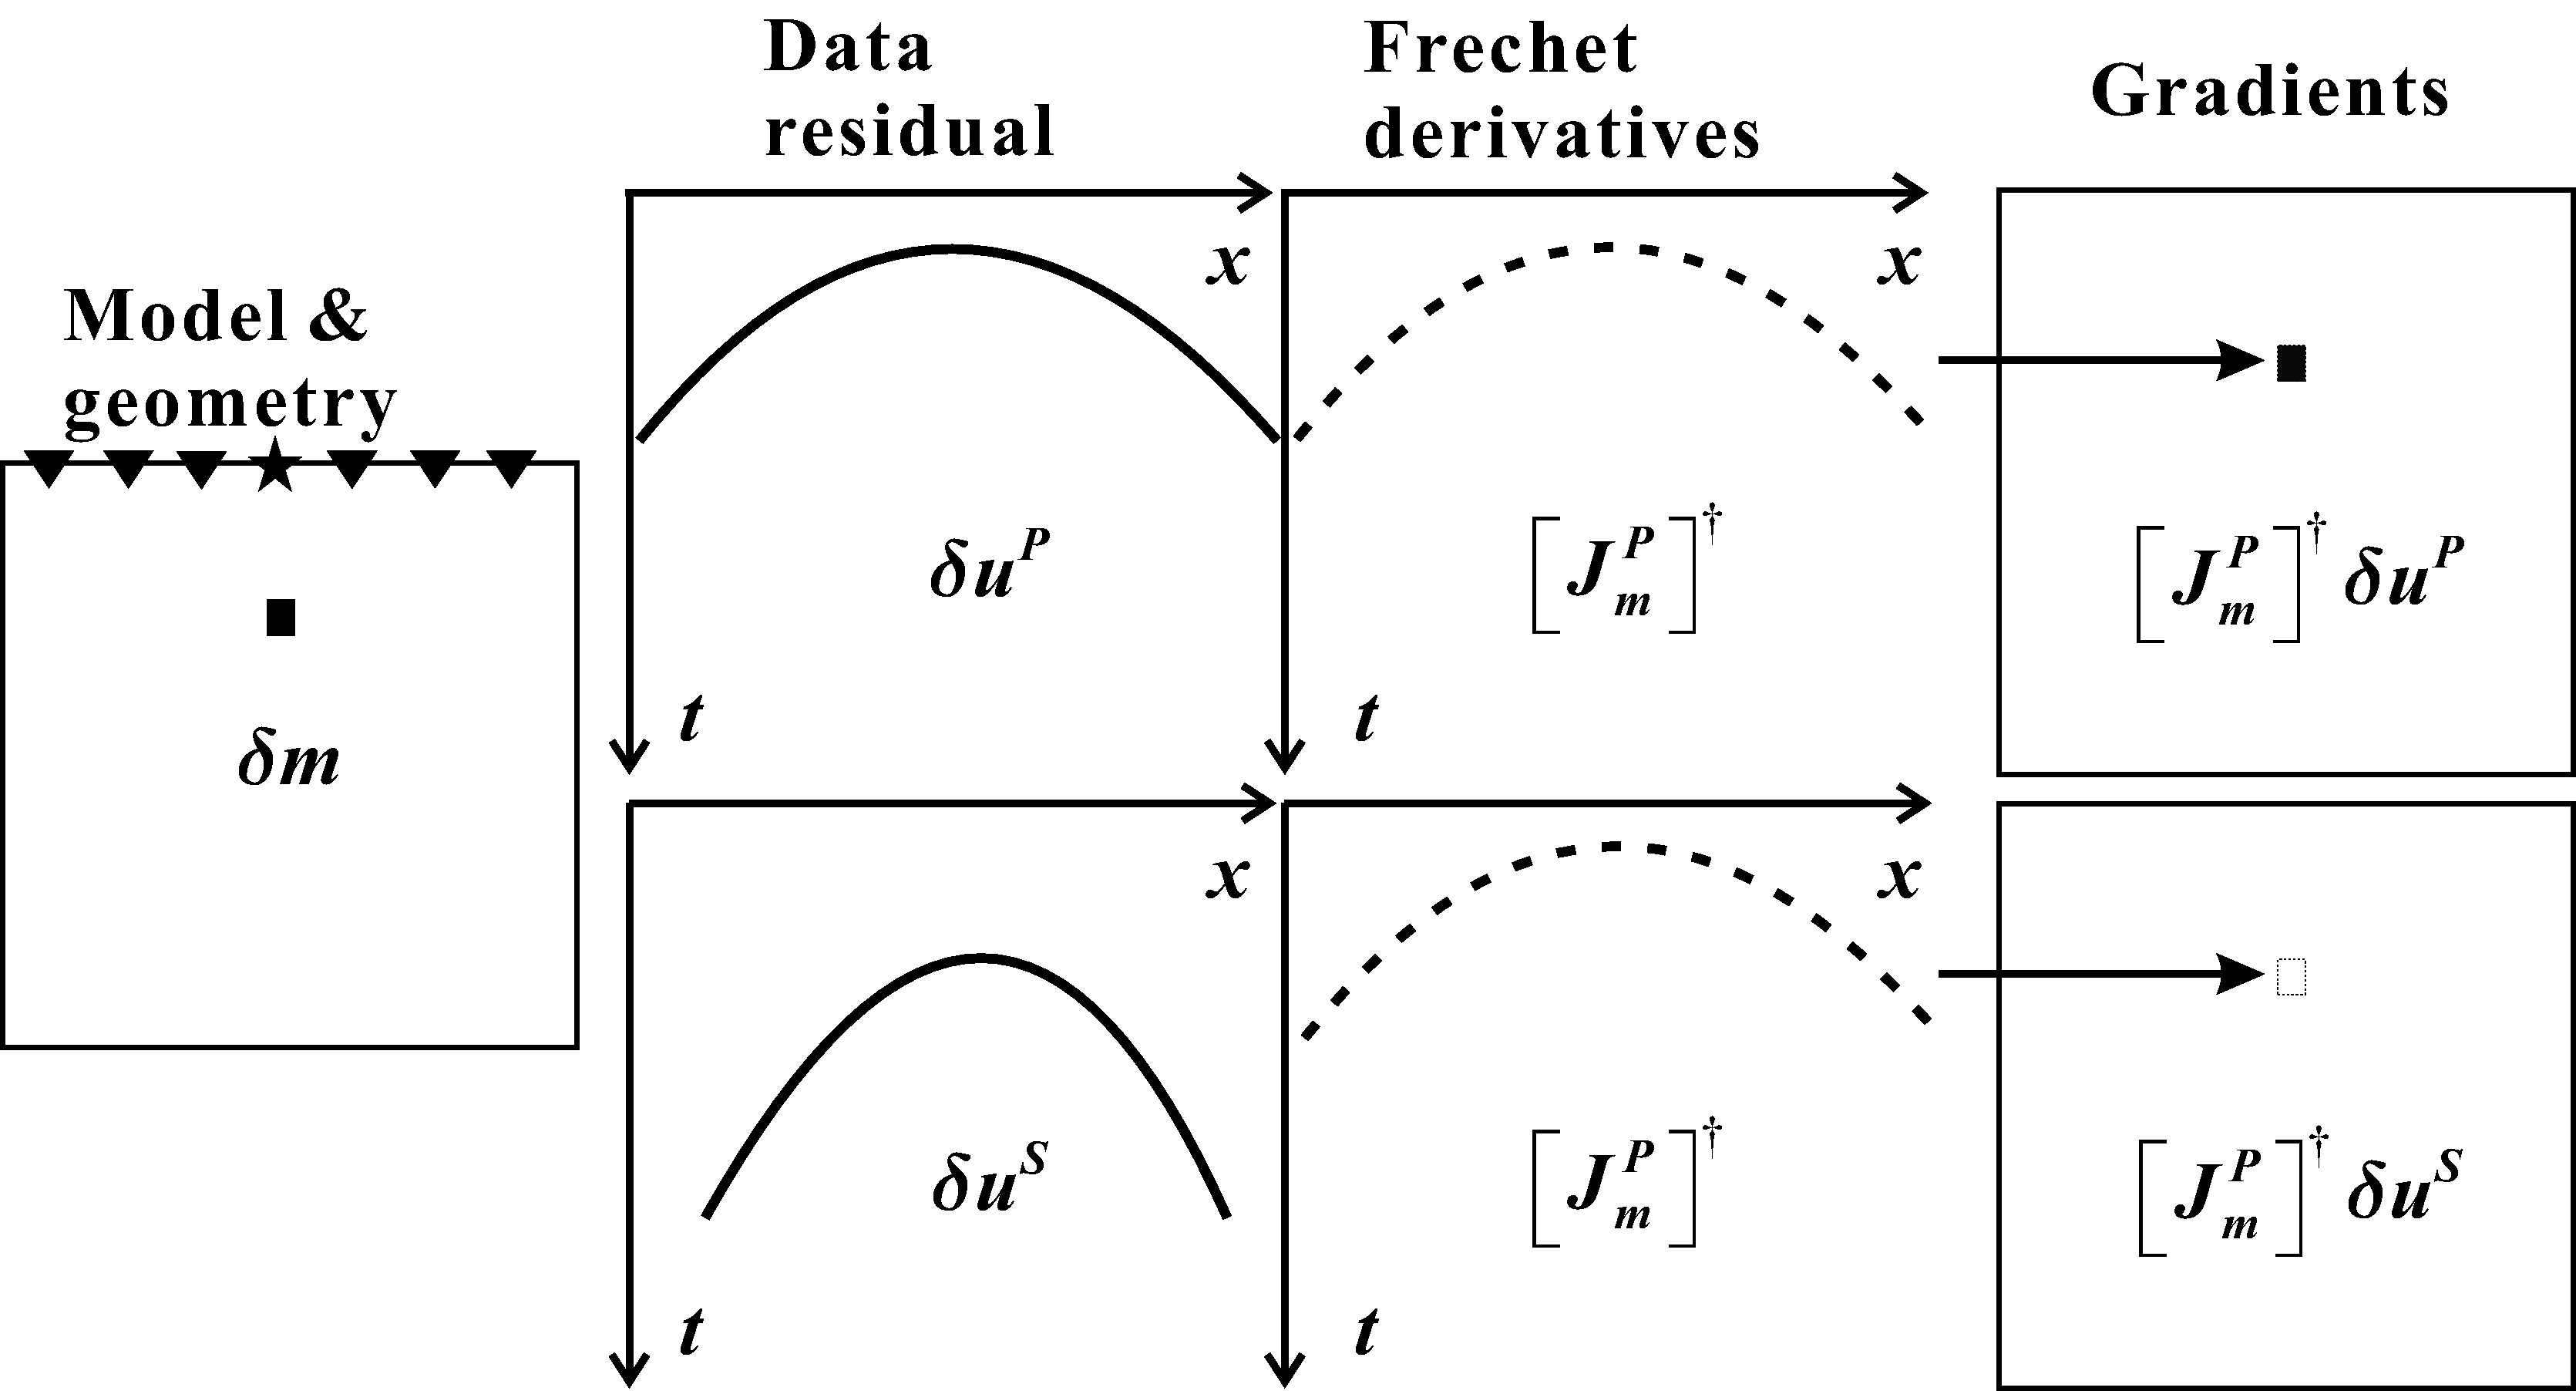
\includegraphics[width=1.0\textwidth]{Figure/chapter02/finalMarmousiII/Fig/zerolagLAST1.pdf}
        \caption{
Schematic illustration of gradient calculation through zero-lag correlation
 between the partial derivative wavefields
and the residual seismogram.
Only a point perturbation is given in the background media for illustration.
    }
    \label{fig:crossterm}
    \end{center}
\end{figure*}

FWI梯度可看作是偏导数波场与数据残差在时间域的零延迟互相关\cite[]{pratt1998gauss}。如图\ref{fig:crossterm}所示,
假设背景介质中有一个点扰动,数据残差为观测数据与模拟数据之间的差值。偏导数波场代表了由于次级源产生的特征性点绕射响应。
一般而言,P波与S波背景速度不同,因而在偏导数波场和地震记录残差中它们的运动学特征也不同(走时和曲率)。
所以,相同波模式之间的零延迟互相关将在梯度计算中占主要能量,而不同波模式之间的互相关则会由于非同相的干涉被基本消除掉。
因此,我们会有以下的交叉项近似:
\begin{equation}
        \begin{split}
                [\mathbf{J}_{V_p}^{S}]^{\dagger}\delta \mathbf{d}^P\approx\mathbf{0},\\
                [\mathbf{J}_{V_s}^{S}]^{\dagger}\delta \mathbf{d}^P\approx\mathbf{0},\\
                [\mathbf{J}_{V_p}^{P}]^{\dagger}\delta \mathbf{d}^S\approx\mathbf{0},\\
                [\mathbf{J}_{V_s}^{P}]^{\dagger}\delta \mathbf{d}^S\approx\mathbf{0},
        \end{split}
        \label{eq:crossterms}
\end{equation}
其中$\mathbf{0}$为空矩阵。
此外,散射模式说明P波速度的扰动不会产生S波散射,所以我们也有:
\begin{equation}
\mathbf{J}^S_{V_p}=\mathbf{0}.
\label{eq:Jsvp}
\end{equation}
从而有:
\begin{equation}
        \begin{split}
[\mathbf{J}^S_{V_p}]^{\dagger}\delta \mathbf{d}^P=\mathbf{0}, \\
[\mathbf{J}^S_{V_p}]^{\dagger}\delta \mathbf{d}^S=\mathbf{0}.
        \end{split}
\label{eq:Jsvp1}
\end{equation}
\subsection{模式解耦梯度预条件}
利用方程\eqref{eq:crossterms}和\eqref{eq:Jsvp1},我们可以获得以下近似:
\begin{equation}
        \mathbf{J}^{\dagger}_{V_p}\delta \mathbf{d}^P\approx
        [\mathbf{J}^P_{V_p}]^{\dagger}\delta \mathbf{d},\quad
        \mathbf{J}^{\dagger}_{V_s}\delta \mathbf{d}^S\approx
        [\mathbf{J}^S_{V_s}]^{\dagger}\delta \mathbf{d}.
        \label{eq:crossterm}
\end{equation}
因此,基于模式解耦的梯度可以表示为:
\begin{equation}
        \begin{pmatrix}
                \mathbf{g}^P_{V_p}\\
                \mathbf{g}^P_{V_s}
        \end{pmatrix}
        \approx\mathfrak{R}\begin{pmatrix}
                [\mathbf{J}_{V_p}^{P}]^{\dagger}\delta \mathbf{d}\\
                [\mathbf{J}_{V_s}^{P}]^{\dagger}\delta \mathbf{d}
        \end{pmatrix},
        \label{eq:MatrixGraP}
\end{equation}
和
\begin{equation}
        \begin{pmatrix}
                \mathbf{g}^S_{V_p}\\ 
                \mathbf{g}^S_{V_s}
        \end{pmatrix}
        \approx\mathfrak{R}\begin{pmatrix}
                \mathbf{0}\\ 
                [\mathbf{J}^S_{V_s}]^{\dagger}\delta \mathbf{d}
        \end{pmatrix}.
        \label{eq:MatrixGraS}
\end{equation}
上述方程表明在梯度计算中可以通过Fr{$\acute{e}$}chet导数的解耦来代替数据残差的解耦。

进一步而言,由于串扰效应主要体现在P波数据中,因此我们舍弃梯度中的$\mathbf{g}_{V_s}^P$项来降低参数耦合效应。
所以我们分别选取解耦后的P波与S波Fr{$\acute{e}$}chet导数来构建$V_p$和$V_s$预条件之后的梯度,也即:
\begin{equation}
        \begin{pmatrix}
                \hat{\mathbf{g}}_{V_p}\\
                \hat{\mathbf{g}}_{V_s}
        \end{pmatrix}=
        \begin{pmatrix}
                \mathbf{g}_{V_p}^P\\
                \mathbf{g}_{V_s}^S
        \end{pmatrix}
        \approx 
        \mathfrak{R}\begin{pmatrix}
                [\mathbf{J}^P_{V_p}]^{\dagger} \delta \mathbf{d}\\
                [\mathbf{J}^S_{V_s}]^{\dagger} \delta \mathbf{d}
        \end{pmatrix}.
        \label{eq:MatrixGraMode}
\end{equation}
这里我们用符号$\hat{}$来指示基于模式解耦的预条件梯度。
最终,EFWI问题转化为通过解耦的方式来迭代求解:
\begin{equation}
        \mathbf{m}_{k+1}=\mathbf{m}_{k}-\alpha_k
        \begin{bmatrix}\mathbf{Q}_1\hat{\mathbf{g}}_{V_p}\\\mathbf{Q}_2\hat{\mathbf{g}}_{V_s}\end{bmatrix}_{k},
        \label{eq:Gradientmethod}
\end{equation}
其中,$\mathbf{Q}_1$和$\mathbf{Q}_2$表示预条件算子。步长$\alpha_k$采用抛物线拟合的方式来搜寻(Vigh
and Starr, 2008\cite[]{vigh20083d})。

\subsection{共轭状态法计算梯度}
显式的计算Fr{$\acute{e}$}chet导数需要进行多达模型网格数量次的正演模拟,这在实际计算中是无法实现\cite[]{virieux2009overview}。
为了避免显式构建Jacobian矩阵,我们采用共轭状态法来计算梯度\cite[]{tromp2005seismic,plessix2006}。利用Green函数的空间互易性,方程\eqref{eq:MatrixGra1}中的原始梯度可以通过正传波场与反传的残差波场之间的时间域
零延迟互相关计算得到:
\begin{equation} 
        \begin{split}
        \mathbf{g}_{V_p}&=-2\rho V_p\int_{0}^{T}\frac{\partial u_i}{\partial
        x_j}\frac{\partial \psi_k}{\partial x_l}
        \delta_{ij}\delta_{kl}dt,\\
        \mathbf{g}_{V_s}&=-2\rho V_s\int_{0}^{T}\frac{\partial u_i}{\partial
        x_j}\frac{\partial \psi_k}{\partial x_l}
        (-2\delta_{ij}\delta_{kl}+\delta_{ik}\delta_{jl}+\delta_{il}\delta_{jk})dt,
        \end{split}
        \label{eq:Gradient_vpvs}
\end{equation}
其中$u_i$是从震源出发的正传波场,$\psi_k$ 是通过数据残差从接收点处反传重建的共轭波场。注意方程\eqref{eq:Gradient_vpvs}
中第一行的算式中自动隐含了正传和共轭波场的散度算子。

从方程\eqref{eq:EquivFre1}可看出,Frech$\acute{e}$t导数的模式解耦等价于施加在散射Green函数上。这就意味着当使用伴随状态法时,
我们只需要解耦伴随波场就可以获得预条件后的梯度,也即:
\begin{equation} 
        \begin{split} 
                \hat{\mathbf{g}}_{V_p}&=-2\rho V_p\int_{0}^{T}\frac{\partial u_i}{\partial
        x_j}\frac{\partial \psi^P_k}{\partial x_l}
        \delta_{ij}\delta_{kl}dt,\\
        &=-2\rho V_p\int_{0}^{T}\frac{\partial u_i}{\partial
        x_j}\frac{\partial \psi_k}{\partial x_l}
        \delta_{ij}\delta_{kl}dt,\\
                \hat{\mathbf{g}}_{V_s}&=-2\rho V_s\int_{0}^{T}\frac{\partial u_i}{\partial
        x_j}\frac{\partial \psi^S_k}{\partial x_l}
        (\delta_{ik}\delta_{jl}+\delta_{il}\delta_{jk})dt,
        \end{split}
        \label{eq:DeGradient_vpvs} 
\end{equation}
其中$\psi^P$和$\psi^S$分别为P波和S波的伴随波场。由于$\mathbf{g}_{V_p}$的计算中隐含了散度算子,总是满足$\hat{\mathbf{g}}_{V_p}=\mathbf{g}_{V_p}$。
对比方程\eqref{eq:Gradient_vpvs},由于S波的散度总是为0,所以在计算预条件后的S波速度梯度时我们舍弃了$-2\delta_{ij}\delta_{kl}$项。
因此,对于P波速度而言,模式解耦已经自动隐含在梯度计算中,但是S波速度的梯度模式解耦预条件需要显式地施加。

解耦伴随波场需要额外的计算量,主要体现在每个时间片中需要两次Fourier变换。为了减少计算量并节省内存消耗,我们
对正传波场与反传波场在时间轴上进行重采样,并且在互相关之前只对反传的伴随波场进行模式解耦。
当更多的多尺度策略考虑进来的时候,也可以对正传波场进行解耦,例如在单级反演中单独的使用S-S或者P-S模式。但是我们并不推荐
这样的策略,我们将在讨论部分进行阐述。
\section{模式解耦降低参数耦合的理论机制}
	在前一节中我们提出了通过模式解耦来第梯度进行预条件的EFWI方式。然而解决参数解耦问题最直接有效(但也最昂贵)
的方法是考虑Hessian矩阵的优化方法。我们将采用解耦后的
Frech$\acute{e}$t导数来调查Hessian和分辨率矩阵的性质,并且对比高斯牛顿梯度与模式解耦方法的梯度来
分析EFWI中模式解耦降低参数耦合的机制。
\subsection{Hessian矩阵及其不同模式的分量}
多参数的Hessian矩阵是一个具有块状结构的对称方阵,其中非对角块测量了不同物理参数的偏导数波场之间的互相关结果,其作用也
是来处理多参数反演中的参数耦合问题。当反问题为近似线性或者数据残差非常小的时候,全Hessian将约等于近似Hessian
$\mathbf{H}_a$\cite[]{pratt1998gauss}:
\begin{equation}
\mathbf{H}_a =\mathfrak{R}[{\mathbf{J}}^{\dagger}\mathbf{J}]. 
\label{eq:hess}
\end{equation}
考虑到Fr{$\acute{e}$}chet导数的解耦(见方程\ref{eq:JPS}),我们可以将 $\mathbf{H}_a$ 分解为四个分量:
\begin{equation}
\begin{split}
\mathbf{H}_a^{PP}=\mathfrak{R}[{\mathbf{J}^{P}}]^{\dagger}[{\mathbf{J}^{P}}],\\
\mathbf{H}_a^{PS}=\mathfrak{R}[{\mathbf{J}^{P}}]^{\dagger}[{\mathbf{J}^{S}}],\\
\mathbf{H}_a^{SP}=\mathfrak{R}[{\mathbf{J}^{S}}]^{\dagger}[{\mathbf{J}^{P}}],\\
\mathbf{H}_a^{SS}=\mathfrak{R}[{\mathbf{J}^{S}}]^{\dagger}[{\mathbf{J}^{S}}].
\end{split}
\label{eq:hessian_component}
\end{equation}

\begin{figure}[!htb]
    \begin{center}
        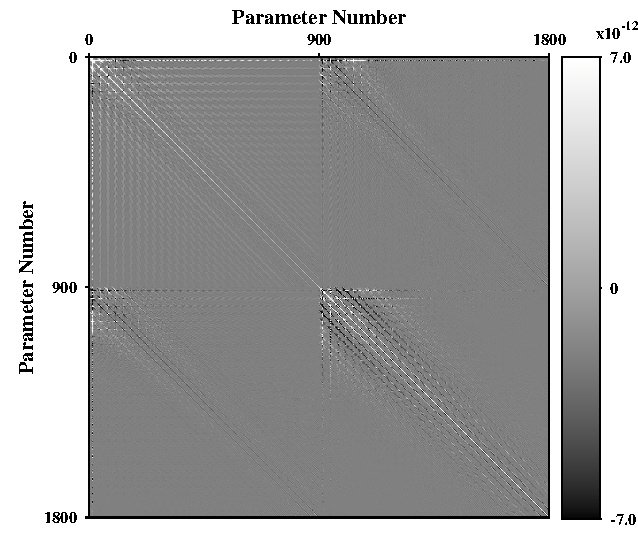
\includegraphics[width=10cm]{Figure/chapter02/ResoOpera/Fig/hessian.pdf}
        \caption{
            近似Hessian矩阵$\mathbf{H}_a$.
    }
    \label{fig:Hessian} 
    \end{center}
\end{figure}
\begin{figure}[!htb]
    \begin{center}
        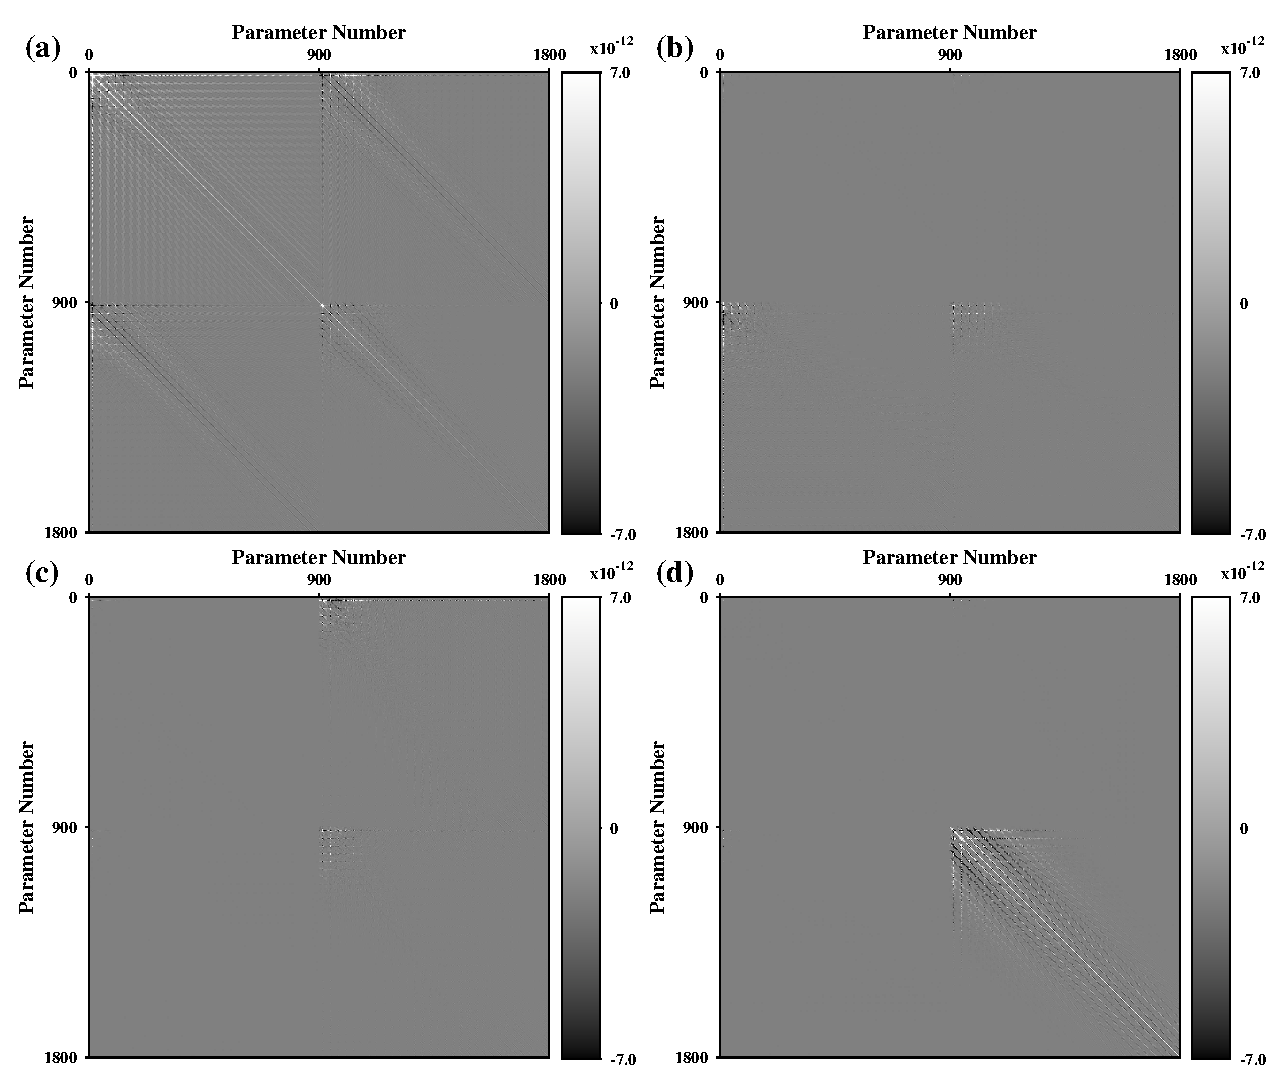
\includegraphics[width=12cm]{Figure/chapter02/ResoOpera/Fig/fourhessian.pdf}
        \caption{
            近似Hessian矩阵的四个分量:
                        (a) $\mathbf{H}_a^{PP}$,
            (b) $\mathbf{H}_a^{PS}$, (c) $\mathbf{H}_a^{SP}$ and (d)$\mathbf{H}_a^{SS}$.
    }
    \label{fig:fourHessian}
    \end{center}
\end{figure}
从应用角度来讲,Hessian矩阵通常是无法计算的。为了调查每个分量各自的贡献,我们在一个网格大小为$30\times30$,
空间采样为5m的模型上数值地计算出Hessian矩阵的各个分量。我们在模型的顶部中央放置一个纯P波震源,接收点分布于四个边界上。
近似Hessian矩阵(图\ref{fig:Hessian})及其分量(图\ref{fig:fourHessian})通过时间域的 Frech{$\acute{e}$}t导数显式求出。近似Hessian矩阵中非对角块中明显的非零元素代表了很强的参数耦合效应。我们可以观察到以下
现象:
首先,交叉项分量,$\mathbf{H}_a^{PS}$ and $\mathbf{H}_a^{SP}$对$\mathbf{H}_a$的贡献可以忽略不计。这是由于相应
的Fr{$\acute{e}$}chet导数因为背景的P波和S波速度不同而不具有相干性。注意到,在这些交叉项分量中会有一些非常小值的非零元素。
这是由于Fr{$\acute{e}$}chet导数中震源附近的异常值所导致。
\begin{equation}
        \mathbf{H}_a\approx
        \mathbf{H}_a^{PP}+
        \mathbf{H}_a^{SS}.
        \label{eq:C3}
\end{equation}
其次,$\mathbf{H}_a$的非对角区块几乎与$\mathbf{H}_a^{PP}$一样,并且$\mathbf{H}_a^{SS}$只有右下的对角快是非零的,这是因为$\mathbf{J}^S=(\mathbf{0}\quad\mathbf{J}^S_{V_s})$。这些现象进一步确认了参数耦合主要是来自P波波场而非S波波场。
\subsection{模型分辨率矩阵及其分量}
通过模式解耦的Frech{$\acute{e}$}t导数对Hessian矩阵的定性分析并不足以理解解耦对反演产生作用的机制。为了评估P波与S波数据对
反演的贡献,我们进一步分析模式解耦如何在模型空间影响分辨率矩阵。模型的分辨率矩阵通常采用Hessian矩阵及其逆矩阵来计算得到
(Menke, 1989\cite[]{menke:1989}; Snieder and Trampert, 1999\cite{snieder1999inverse})。方程\eqref{eq:finalMatrixshort}对应的反问题,我们采用以下公式来更新模型:
\begin{equation}
	\delta \tilde{\mathbf{m}}=-\mathbf{H}^{-1}_a\mathbf{J}^{\dagger}\delta 
        \mathbf{d},
        \label{eq:LeastSol}
\end{equation}
其中$\delta\tilde{\mathbf{m}}$为用全部数据残差估计得到的模型扰动。根据Born近似$\delta\mathbf{d}=\mathfrak{F}{\delta\mathbf{u}}$,
然后将方程\eqref{eq:finalMatrixshort}带入到式\eqref{eq:LeastSol}中,并省略采样函数$\mathfrak{F}$,可以有:
\begin{equation}
	\delta \tilde{\mathbf{m}}=\mathbf{R}\delta \mathbf{m},
	\label{eq:ResoMatr}
\end{equation}
其中$\delta \mathbf{m}$表示真实模型扰动,且模型分辨率矩阵$\mathbf{R}$满足:
\begin{equation}
        \mathbf{R}=-\mathbf{H}^{-g}_a\mathbf{H}_a. 
        \label{eq:ResoOper} 
\end{equation}
注意,由于有限的观测导致近似Hessian总是病态的,因此这里我们采用Hessian的伪逆(广义逆)$\mathbf{H}^{-g}_a$,而不是$\mathbf{H}^{-1}_a$。

\begin{figure*}
    \begin{center}
        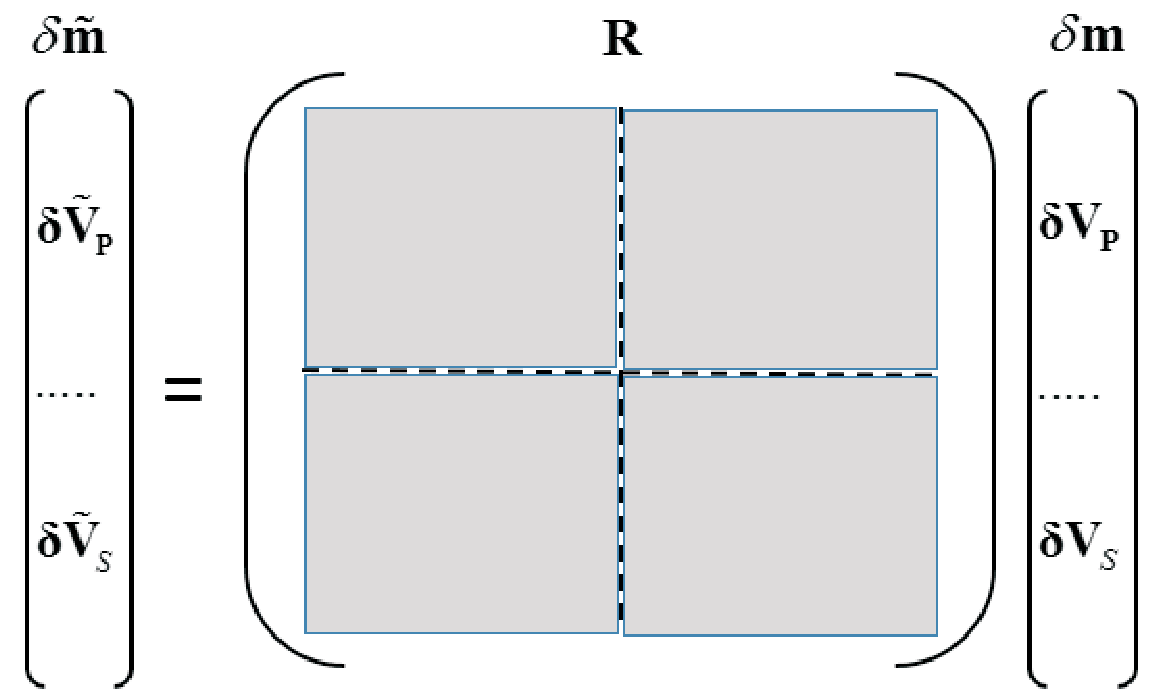
\includegraphics[width=10cm]{Figure/chapter02/ResoOpera/Fig/resolutionmatrix.pdf}
        \caption{
			分辨率矩阵示意图。对于双参数的反问题,分辨率矩阵可以分成四个区块。
    }
    \label{fig:IllustrReso}
    \end{center}
\end{figure*}
如图\ref{fig:IllustrReso}所示,模型分辨率矩阵可看作是作用在真实模型上的滤波器。如果观测手段足够好,则分辨率矩阵会是严格的单位矩阵,
也即$\mathbf{R}=\mathbf{I}$,那么模型参数也会是唯一确定的。然而通常情况下$\mathbf{R} \ne \mathbf{I}$,因此对模型的估计将是真实模型参数的加权平均值。
$\mathbf{R}$ 的对角区块隐含了单参数内部间的相互影响及其相应的分辨能力,而非对角区块则表明了不同参数之间的相互作用。如果对角区块上有明显的非零元素分布,
则预示着不可忽视的参数耦合效应。我们如果采用分解后的P波数据,则方程\eqref{eq:LeastSol} 变为:
\begin{equation}
        \delta \tilde{\mathbf{m}}^P=-\mathbf{H}^{-1}_a\mathbf{J}^{\dagger}\delta \mathbf{d}^P,
        \label{eq:LeastSolP}
\end{equation}
其中$\delta \tilde{\mathbf{m}}^P$ 表示P波数据给出的模型估计。同样采用式\eqref{eq:LeastSol}-\eqref{eq:ResoOper}的推导,
我们可以获得P波数据的模型分辨率矩阵:
\begin{equation}
        \mathbf{R}^P=-\mathbf{H}^{-g}_a\mathbf{H}_a^P,
        \label{eq:ResoOperP}
\end{equation}
其中$\mathbf{H}_a^P=\mathbf{J}^{\dagger}\mathbf{J}^P$。类似的,S波的分辨率矩阵为:
\begin{equation}
        \mathbf{R}^S=-\mathbf{H}^{-g}_a\mathbf{H}_a^S,
        \label{eq:ResoOperS}
\end{equation}
且$\mathbf{H}_a^S=\mathbf{J}^{\dagger}\mathbf{J}^S$。容易证明$\mathbf{R}=\mathbf{R}^P+\mathbf{R}^S$。

\begin{figure}[!htb]
    \begin{center}
        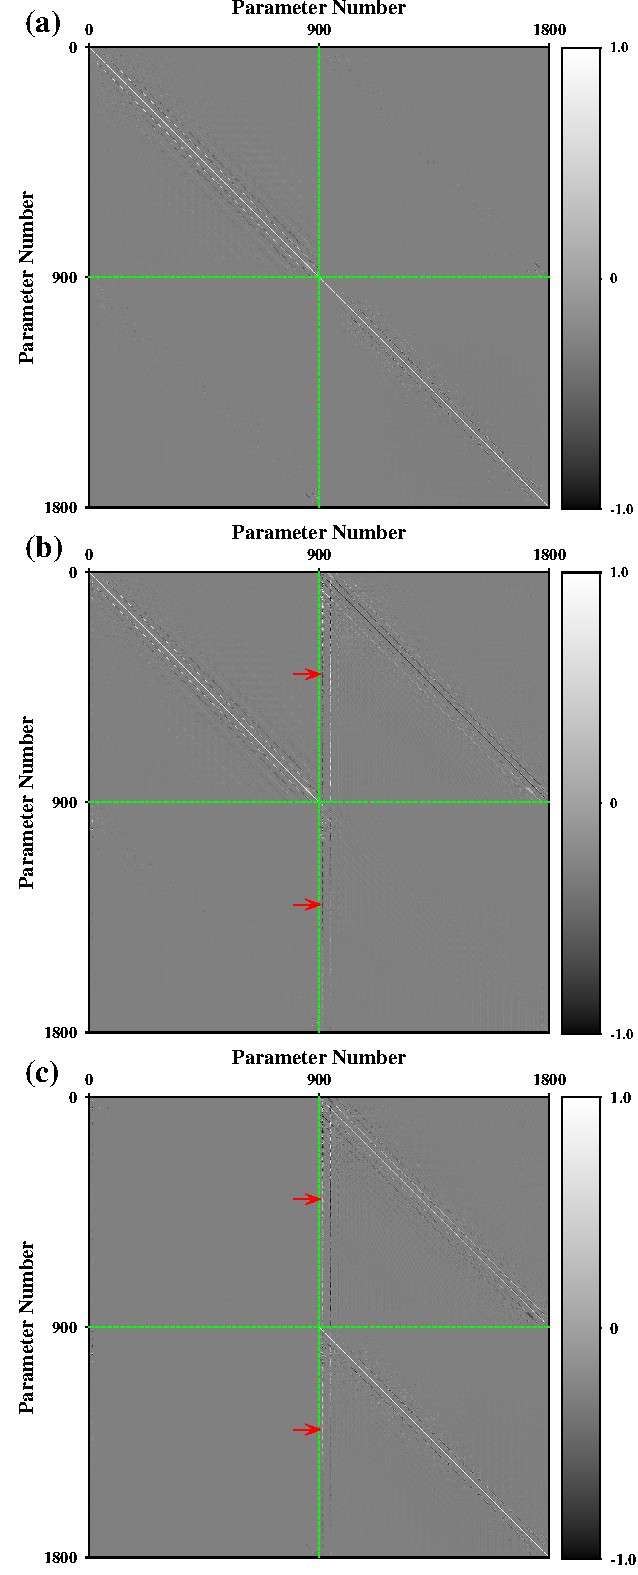
\includegraphics[width=8cm]{Figure/chapter02/ResoOpera/Fig/resolutionoriginal.pdf}
        \caption{
Resolution matrix and its components:
(a) $\mathbf{R}$, (b) $\mathbf{R}^P$ and (c) $\mathbf{R}^S$.
    }
    \label{fig:Resolution}
    \end{center}
\end{figure}
同样采用前文所述小模型试验,我们可以显式计算出模型分辨率矩阵$\mathbf{R}$,$\mathbf{R}^P$和$\mathbf{R}^S$。
原始分辨率矩阵(图\ref{fig:Resolution}a)为带状对角阵,对角元素为小于1的正值。这说明了近似Hessian的逆可以为$V_p$和$V_s$的反演
提供很好的预条件。P波与S波数据对应的分辨率矩阵(图\ref{fig:Resolution}b和c)展示了一些有趣的现象。例如,$\mathbf{R}^P$和$\mathbf{R}^S$的非零对角块
构成了$\mathbf{R}$。除了一些由于震源附近的干扰而导致的假象,$\mathbf{R}^P$的底部两个区块都为空矩阵。在$\mathbf{R}^P$和$\mathbf{R}^S$的右上区块,其中的元素值
大小相等符号相反,两者相加为零从而能够使得$\mathbf{R}$右上区块为空。这些特征说明,对与线性的反问题(无cycle-skipping),P波与S波都对反演$V_p$有贡献,
而P波对$V_s$的贡献非常弱。常规的梯度法由于只用P波数据来计算$V_p$梯度(见式\ref{eq:Gradient_vpvs}),而这部分P波数据有可能来自$V_s$扰动,从而导致反演受到
参数耦合的影响。此外,单独用S波数据可以很好的分辨$V_s$。模式解耦的预条件方式利用了上述特征,因而其能够压制反演中参数间的耦合。
\subsection{与Gauss-Newton梯度的比较}
GN方法利用近似Hessian的逆对梯度进行预条件来处理参数之间的耦合效应:
\begin{equation}
\delta\tilde{\mathbf{m}} = - \mathbf{H}^{-1}_a\mathbf{g}.
\label{eq:GN}
\end{equation}
假设$\mathbf{H}_a$的伪逆为:
\begin{equation}
        \mathbf{H}^{-g}_a=    
        \begin{bmatrix}
                \mathbf{D}&\mathbf{E} \\
                \mathbf{F}&\mathbf{G}
        \end{bmatrix},
        \label{eq:HessInv}
\end{equation}
则GN方法实际上利用以下公式来更新模型:
\begin{equation}
    \mathbf{{m}}_{k+1}
    =\mathbf{{m}}_{k}-\alpha_k 
    \begin{bmatrix}
        \mathbf{D}\mathbf{g}^P_{V_p} +
        \mathbf{E}\mathbf{g}^P_{V_s}+
        \mathbf{E}\mathbf{g}^S_{V_s}\\
        \mathbf{G}\mathbf{g}^S_{V_s}
    \end{bmatrix}_{k},
    \label{eq:PreGNFi}
\end{equation}
因为
\begin{equation}
        \delta \mathbf{V}^P_s\approx0, \quad \delta \mathbf{V}_s \approx \delta
        \mathbf{V}^S_s=-\mathbf{G}\mathbf{g}^S_{V_s},
        \label{eq:KeyPoint}
\end{equation}
(见附录A)。
\begin{figure}[!htb]
    \begin{center}
        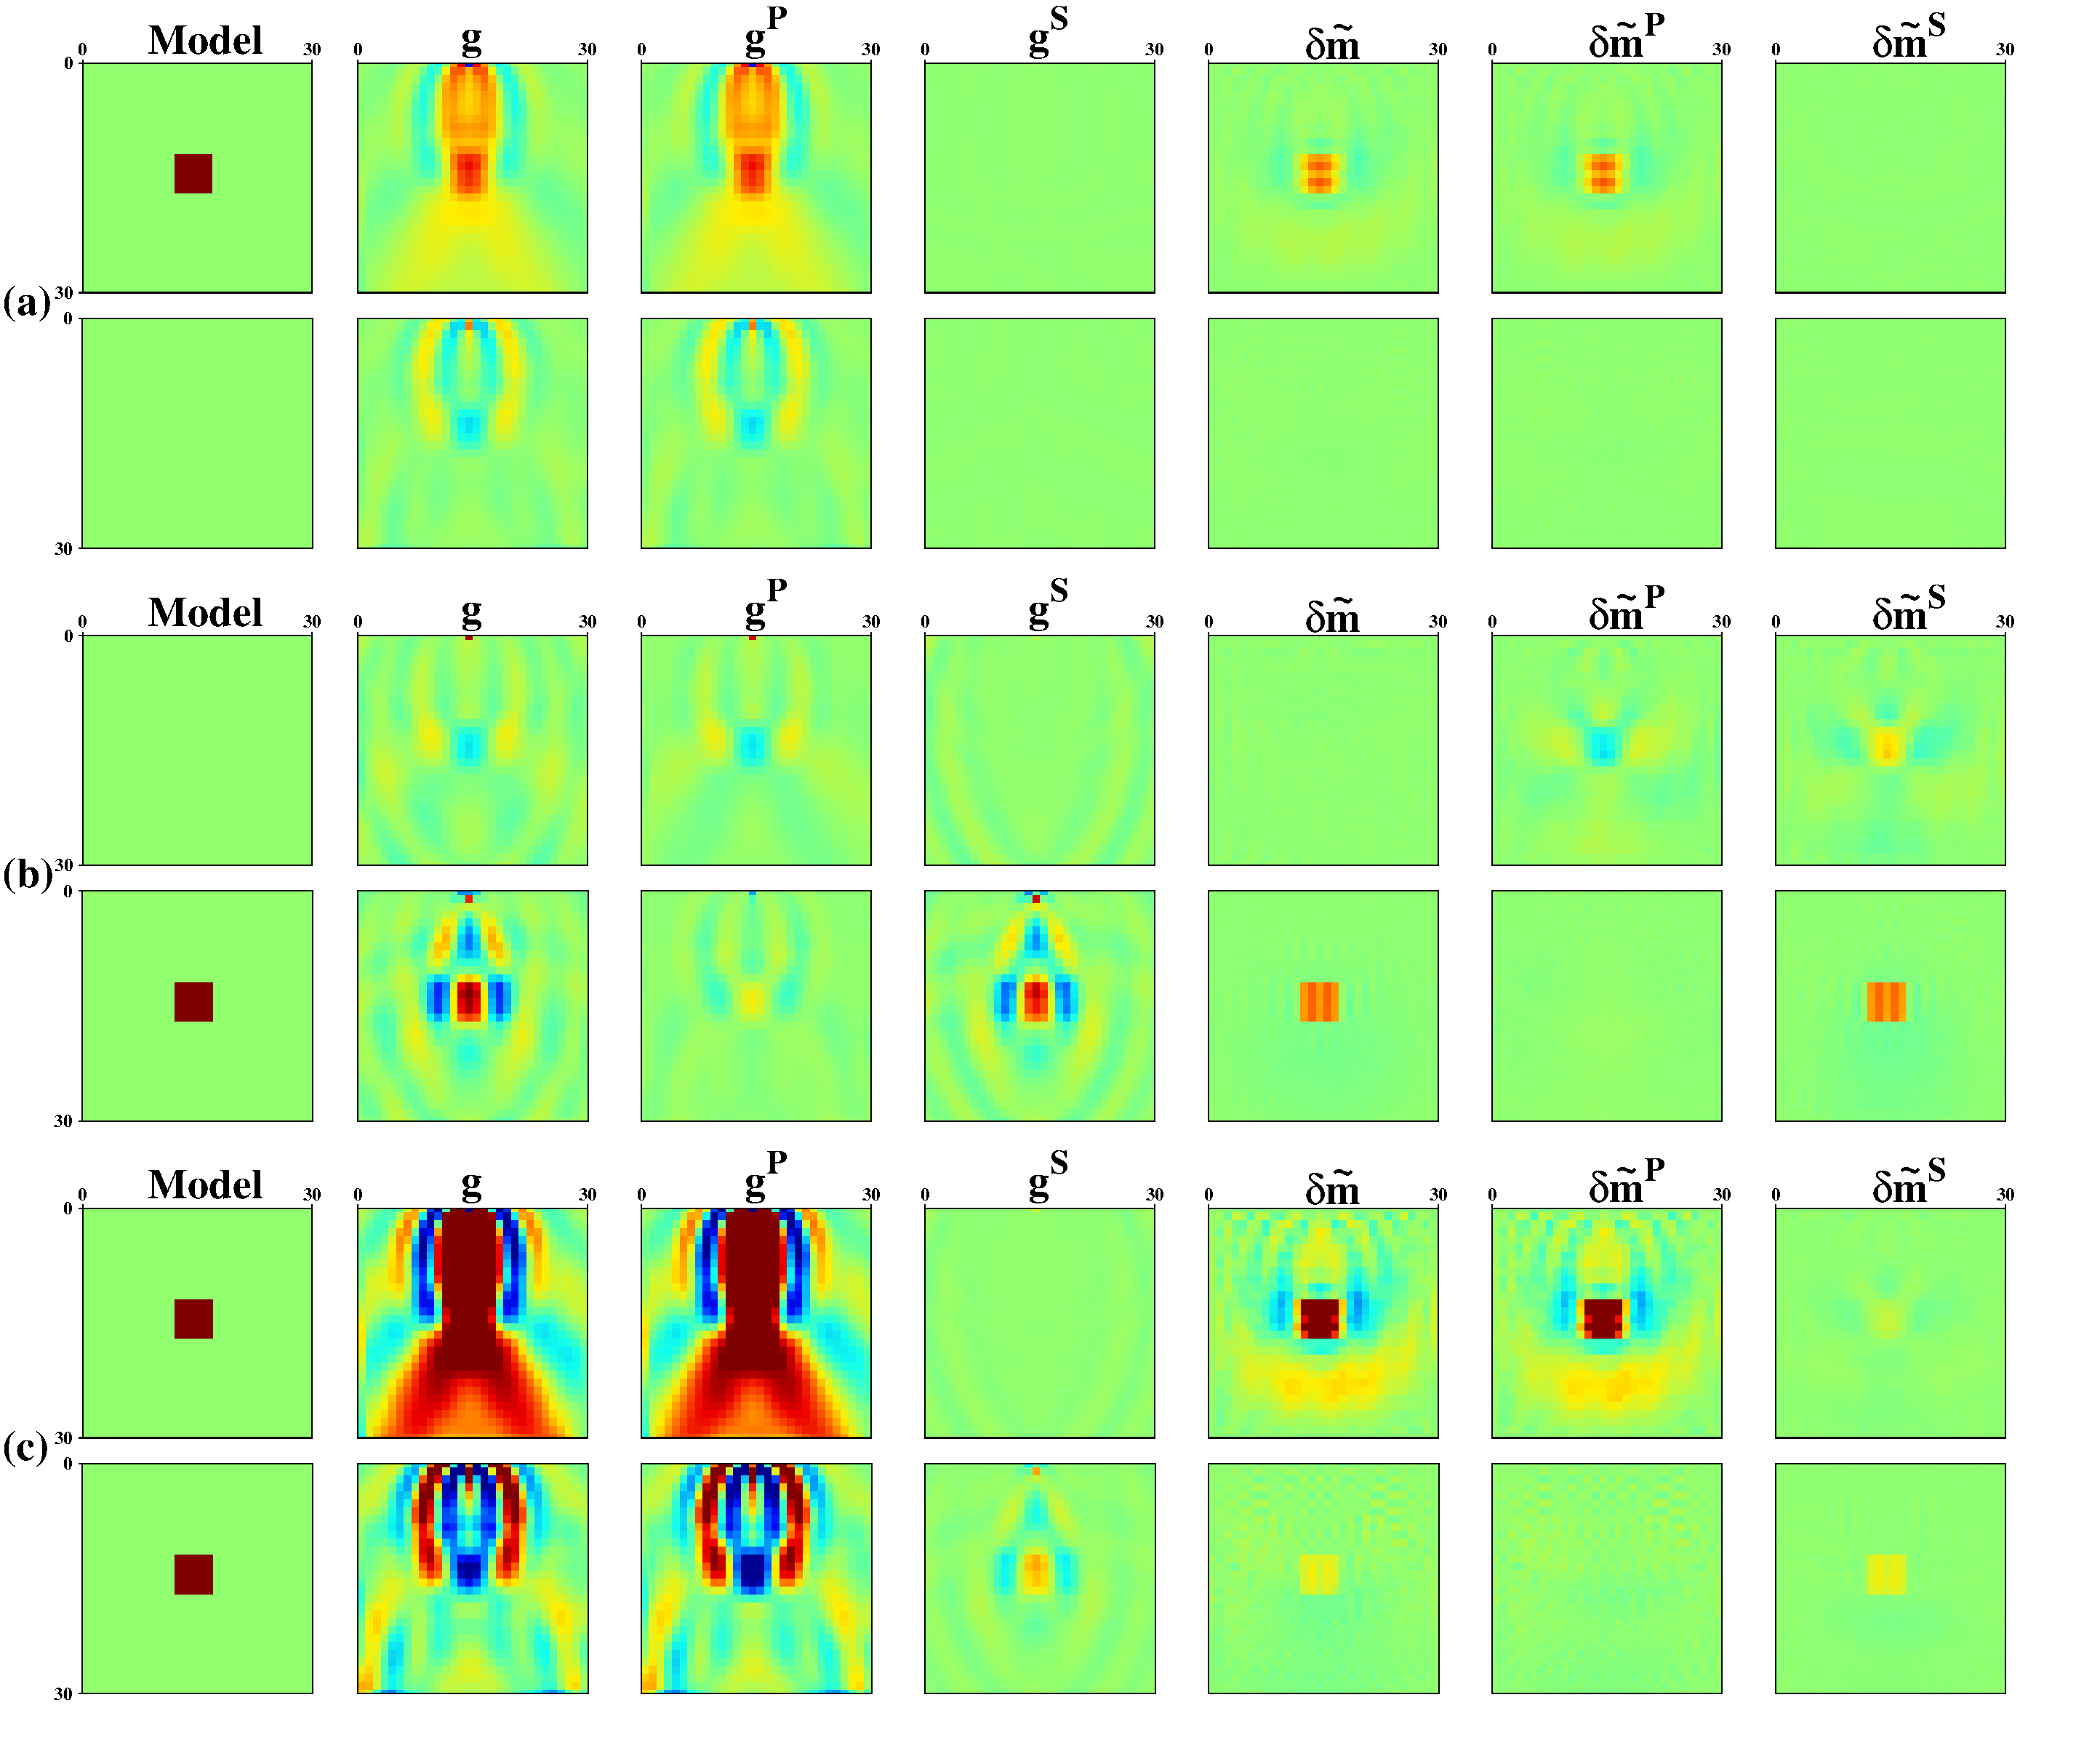
\includegraphics[width=14cm]{Figure/chapter02/Hessiantest/Fig/newepsall.pdf}
        \caption{
			原始方法、GN方法以及模式解耦的第一次迭代梯度之间的对比。
    (a) $\delta V_p \neq 0$, $\delta V_s=0$; (b) $\delta V_p=0$, $\delta V_s\neq0$; and (c)
    $\delta V_p=10 \delta V_s$.
	从上到下为三个面板,每个面板中包含2行7列。第一行对应$V_p$,
	第二行对应$V_s$。7列从左到右依次为真实模型$\mathbf{m}=(\mathbf{V}_p,
    \mathbf{V}_s)$;
    原始梯度$\mathbf{g}=(\mathbf{g}_{V_p},\mathbf{g}_{V_s})$,
    $\mathbf{g}^P=(\mathbf{g}^P_{V_p},\mathbf{g}^P_{V_s})$,
    $\mathbf{g^S}=(\mathbf{g}^S_{V_p},\mathbf{g}^S_{V_s})$;
    GN 梯度$\delta
    \tilde{\mathbf{m}}=(\delta\tilde{\mathbf{V}}_p,\delta\tilde{\mathbf{V}}_s)$;
        模式解耦预条件梯度$\delta
        \tilde{\mathbf{m}}^P=(\delta\tilde{\mathbf{V}}^P_p,\delta\tilde{\mathbf{V}}^P_s)$
         $\delta
        \tilde{\mathbf{m}}^S=(\delta\tilde{\mathbf{V}}^S_p,\delta\tilde{\mathbf{V}}^S_s)$。
    }
    \label{fig:all}
    \end{center}
\end{figure}
在图\ref{fig:all}中,我们同样采用前文中小模型实验来比较原始梯度、GN梯度和解耦梯度。
我们在模型中央放置三种不同类型、大小为10$\times$10m的参数扰动组合,分别为:(a) $\delta V_p \neq 0$, $\delta V_s = 0$; (b) $\delta V_p = 0$,
$\delta V_s \neq 0$,和(c) $\delta V_p =10\delta
V_s$。初始模型为均匀的背景速度。在第一组实验中只有P波数据,我们可以看到原始的梯度,$\mathbf{g}_{V_p}$和$\mathbf{g}_{V_s}$中,有非常明显的参数耦合效应。
从图\ref{fig:all}a和b中可以看到,对于物理参数A而言,另一个参数B扰动会产生一个与B扰动方向相反的A的梯度。从图\ref{fig:all}b和c中$\mathbf{g}^{P}_{V_s}$看到,尽管P波数据残差可能携带了$\delta V_s$的信息,
常规梯度类方法用P波数据来反演$V_s$将会受到参数耦合的影响。在第三组实验中,由于参数耦合的影响,$\mathbf{g}^P_{V_s}$甚至提供了错误的更新方向。
而由于S波残差只与$\delta
V_s$有关,因此正如我们所期望的,$\mathbf{g}^S_{V_s}$总是能提供一个正确的更新方向。所以,$\mathbf{g}^P_{V_s}$是梯度参数耦合部分的主要能量。
一般来说,在以P波能量占主导的地震数据中,梯度的参数耦合部分总是带来负面的效应,除非有行之有效的预条件算子,例如图\ref{fig:all}中的GN梯度。

更重要的是,图\ref{fig:all}中最后三列结果在数值上验证了方程\eqref{eq:KeyPoint},同时也展示了模式解耦梯度法与GN方法之间的异同。与常规梯度法不同,
GN方法利用Hessian的逆以不同权重叠加三个解耦之后的梯度,
$\mathbf{g}^P_{V_p}$、$\mathbf{g}^P_{V_s}$和$\mathbf{g}^S_{V_s}$,来获得P波速度梯度的最佳预条件。对于S波速度,GN方法实际上用
$\mathbf{G}$做为算子来对S波数据梯度做预条件处理。而算子$\mathbf{G}$近似等价于$[\mathbf{J}^{S}_{V_s}]^{\dagger}\mathbf{J}^{S}_{V_s}$的伪逆,
见方程\ref{eq:ResoOperS2}。正如方程\eqref{eq:Gradientmethod}所示,模式解耦梯度法也需要进一步的预条件来加速收敛。例如,预条件算子$\mathbf{Q}_2$
只需要达到解决S波的照明补偿以及子波带宽效应即可,也即近似$\mathbf{G}$的效果。因此,对
$V_s$反演,模式解耦梯度法几乎可看作是采用解耦的S波数据进行的单参数反演。所以预条件算子$\mathbf{Q}_2$要更廉价一些,比如利用单参数拟Hessian或者l-BFGS
方法。这种预条件方法为$V_s$反演近似提供了GN梯度同时降低了迭代中的参数耦合,因而其能够在不计算Hessian情况下加速收敛。

\section{数值实验}
本节中,我们用两个理论数据的例子来验证模式解耦EFWI的有效性,同时与常规梯度法的反演结果进行对比。实验中我们采用纯P波震源来合成多分量地震记录。
从较好的初始模型开始,$V_p$和$V_s$将同时被反演。我们在时间域对数据进行低通滤波,然后采用从低频到高频的多尺度策略来避免陷入局部极值。因此,反演
分为四个不同的阶段:0-2Hz,0-4Hz,0-6Hz和0-10Hz。为简单起见,原始梯度法与解耦的梯度法都采用了随深度变化的照明补偿预条件算子\cite[]{kohn:2012}。
\subsection{流体饱和模型}
图\ref{fig:smallmodel}中,我们定义了一个在沙岩背景模型中的流体饱和储层,背景模型参数为$V_p=3.14 km/s$, $V_s=1.56 km/s$以及$\rho=2000 kg/m^{-3}$。储层的上部为气饱和,参数为
$V_p=2.6 km/s$和$V_s=1.66 km/s$,下部为水饱和$V_p=3.0 km/s$和$V_s=1.66 km/s$。
储层的速度值根据沙岩物理模型给出\cite[]{mavko2009rock}。在模型表面,我们合成32炮数据,炮间距为100m,每炮数据为400道记录,道间距为10m。反演从背景模型开始。
每阶段最大迭代次数限制为10次。从反演结果上看,常规EFWI方法能得到可接受的$V_p$模型,而$V_s$反演结果由于很强的参数耦合影响则非常糟糕。
由于在初始阶段,梯度会受到参数耦合的强烈影响,这导致模型中长波长成分的重建受到严重干扰,因此在有限的迭代次数下反演最终收敛到了局部极值中。
但是,因为采用了模式解耦之后的梯度,MD方法最后很好的重建了$V_p$ 和$V_s$模型。
\begin{figure}[!htb]
    \begin{center}
		\subfloat[]{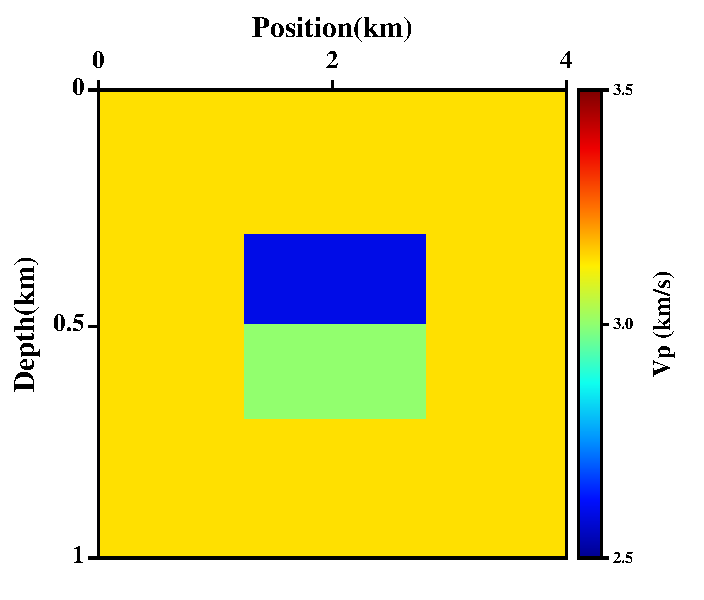
\includegraphics[width=5cm]{Figure/chapter02/smallmodel/Fig/truevp.pdf}}
		\subfloat[]{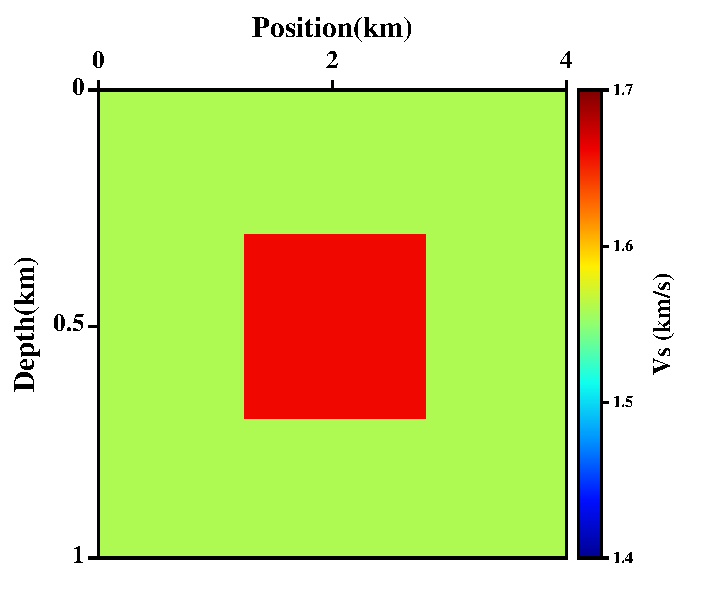
\includegraphics[width=5cm]{Figure/chapter02/smallmodel/Fig/truevs.pdf}}\\
		\subfloat[]{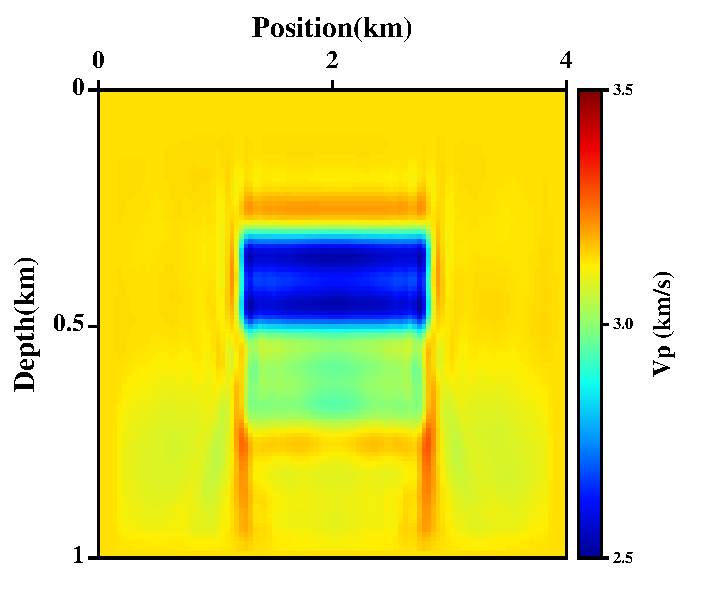
\includegraphics[width=5cm]{Figure/chapter02/smallmodel/Fig/nodecomvp.pdf}}
		\subfloat[]{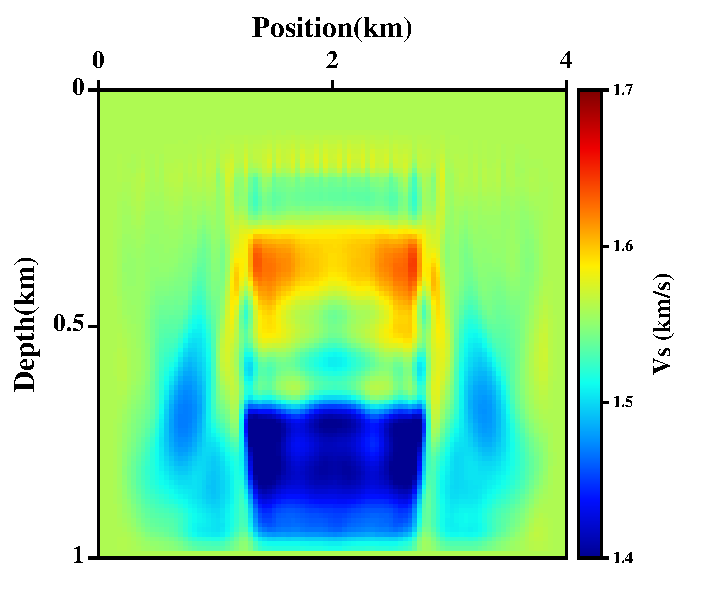
\includegraphics[width=5cm]{Figure/chapter02/smallmodel/Fig/nodecomvs.pdf}}\\
		\subfloat[]{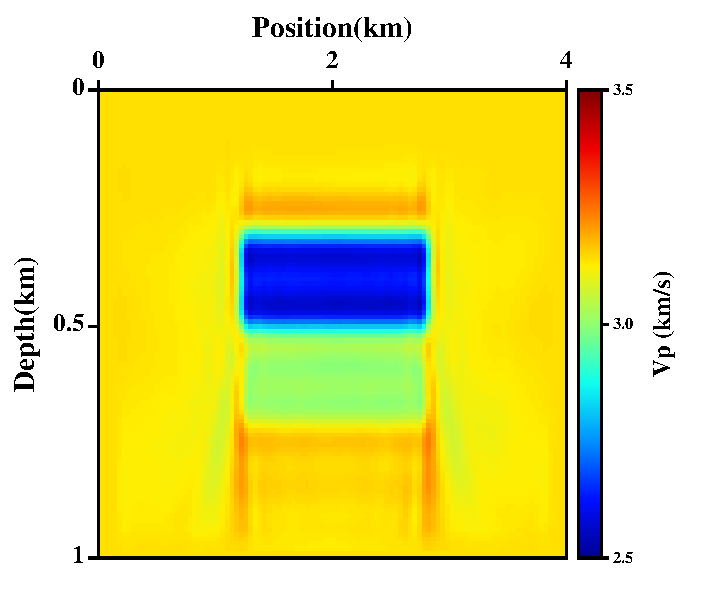
\includegraphics[width=5cm]{Figure/chapter02/smallmodel/Fig/decomvp.pdf}}
		\subfloat[]{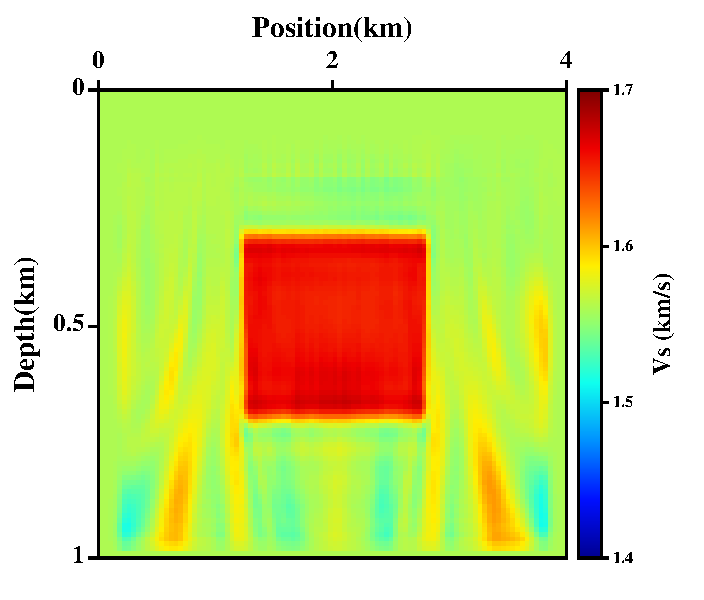
\includegraphics[width=5cm]{Figure/chapter02/smallmodel/Fig/decomvs.pdf}}
        \caption{
			流体饱和沙岩模型的EFWI结果:左侧为$V_p$,右侧为$V_s$;
			(a),(b)为真实模型;(c),(d)为PCG方法反演结果; (e), (f)为模式解耦方法反演结果。
    }
    \label{fig:smallmodel}
    \end{center}
\end{figure}
\subsection{Marmousi-II模型}
\begin{figure}[!htb]
    \begin{center}
		\subfloat[]{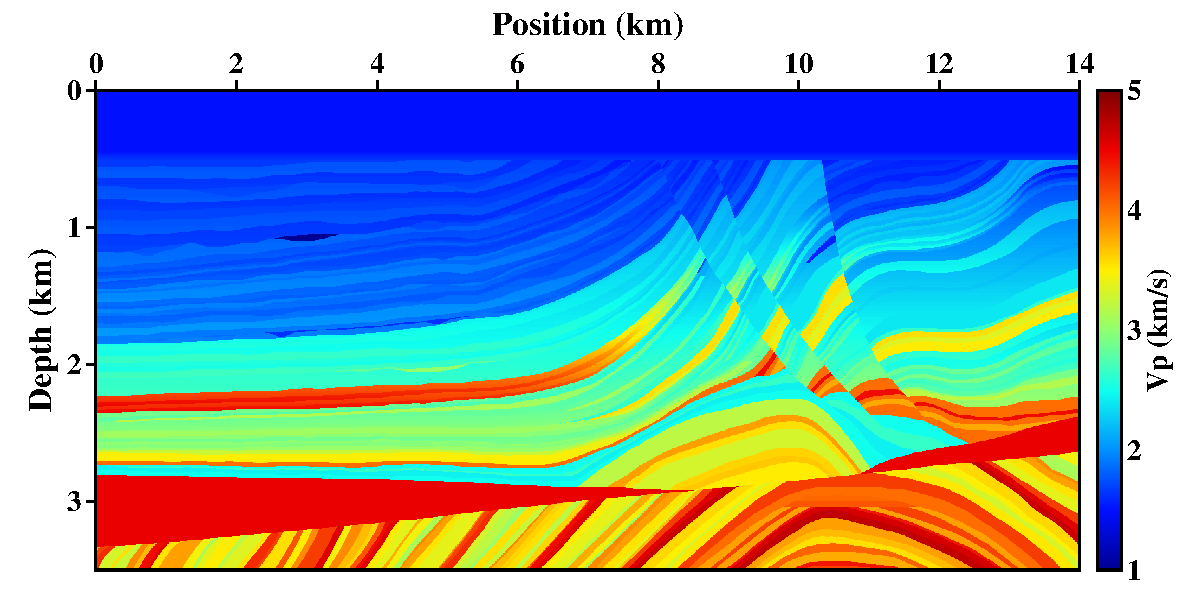
\includegraphics[width=7cm]{Figure/chapter02/tariqsugresult/Fig/truevp.pdf}}
		\subfloat[]{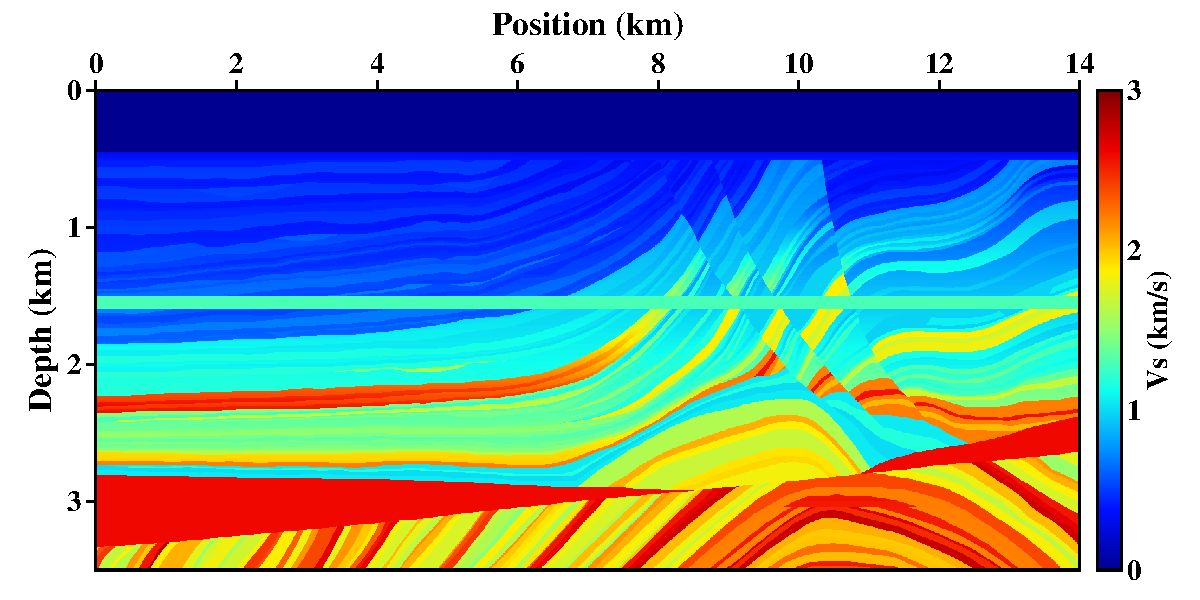
\includegraphics[width=7cm]{Figure/chapter02/tariqsugresult/Fig/truevs.pdf}}\\
		\subfloat[]{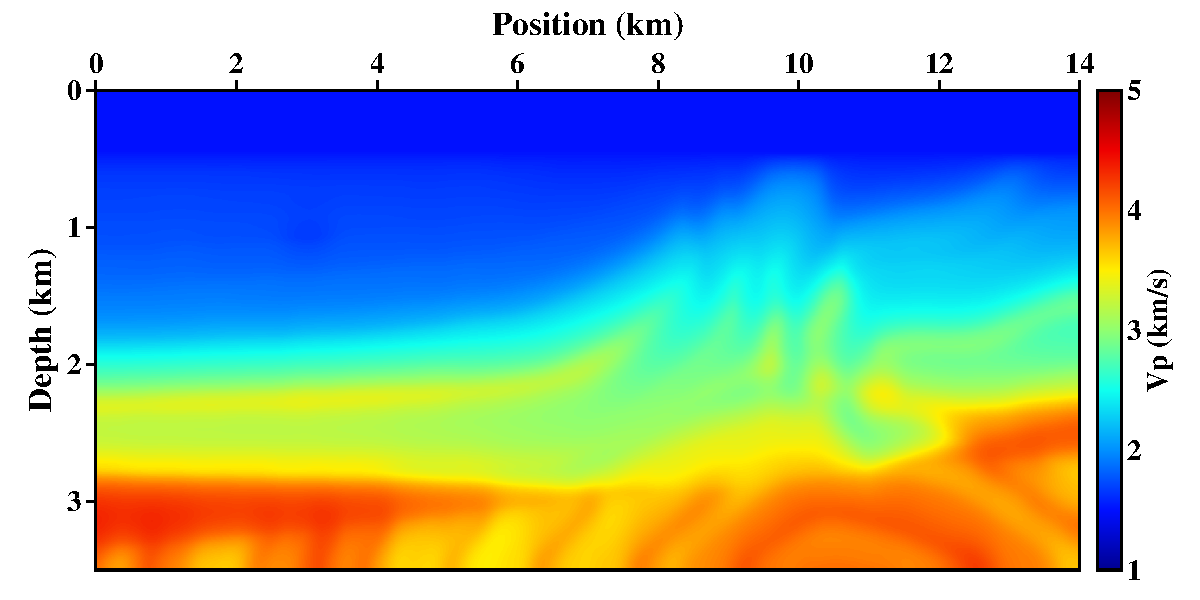
\includegraphics[width=7cm]{Figure/chapter02/tariqsugresult/Fig/initvp.pdf}}
		\subfloat[]{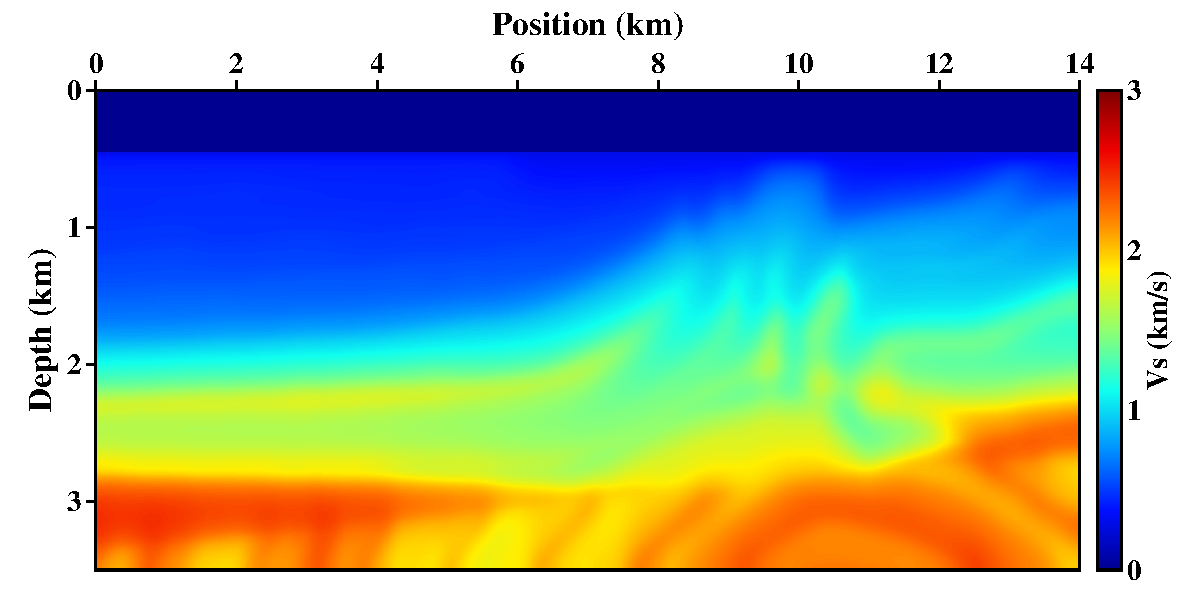
\includegraphics[width=7cm]{Figure/chapter02/tariqsugresult/Fig/initvs.pdf}}
        \caption{
			SEG Marmousii-II模型:(a), (b)分别为真实的$V_p$和$V_s$模型; (c),
			(d)分别为初始的$V_p$和$V_s$模型。注意,P波速度含有含气沙岩储层产生的速度异常以及S波速度
			中加入了高速薄层异常结构。
    }
    \label{fig:MarInitTrue}
    \end{center}
\end{figure}
\begin{figure}[!htb]
    \begin{center}
		\subfloat[]{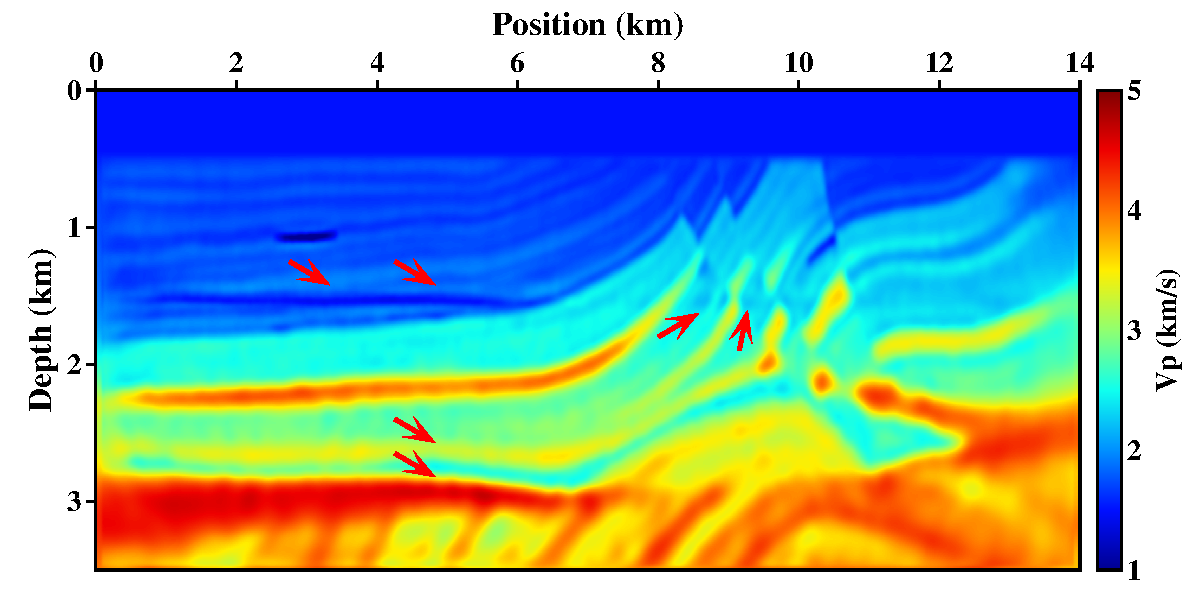
\includegraphics[width=7cm]{Figure/chapter02/tariqsugresult/Fig/nodevp.pdf}}
		\subfloat[]{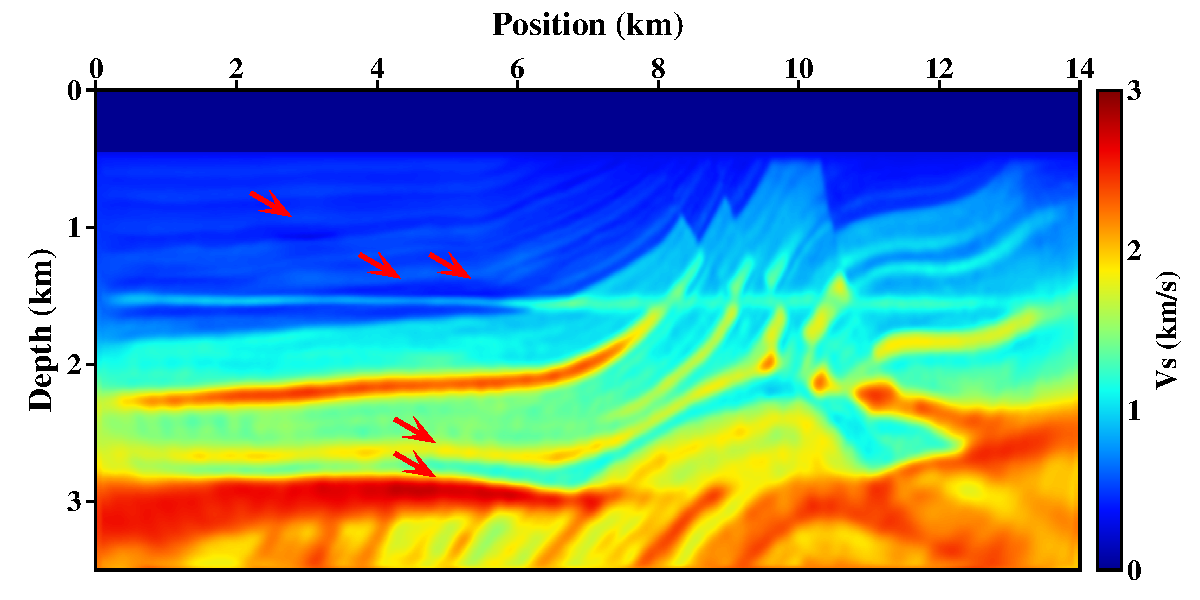
\includegraphics[width=7cm]{Figure/chapter02/tariqsugresult/Fig/nodevs.pdf}}\\
		\subfloat[]{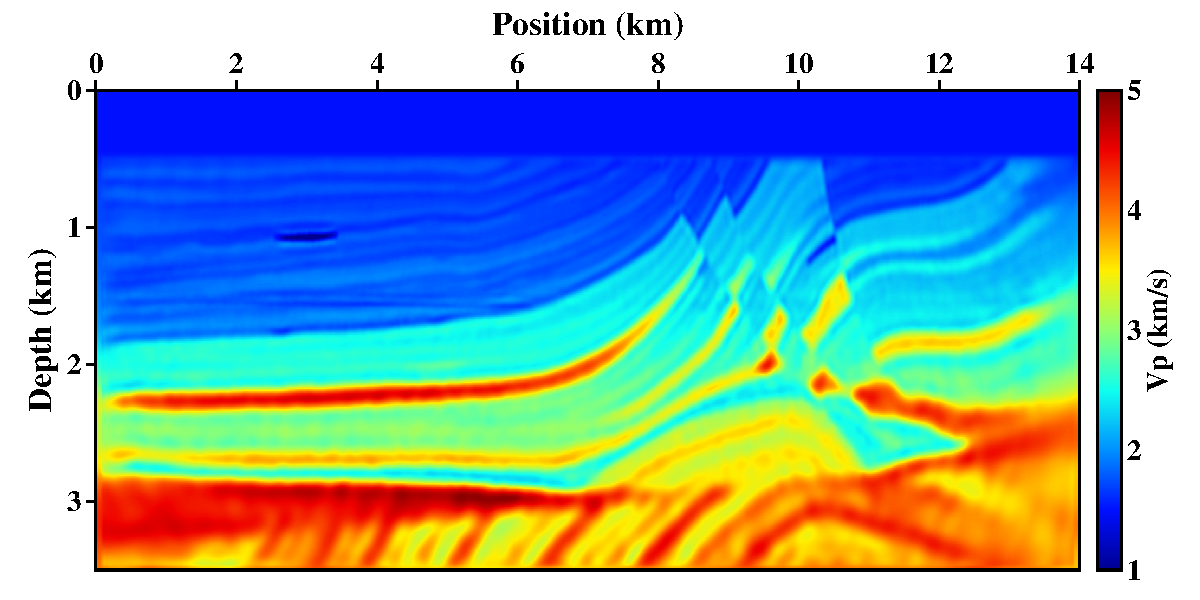
\includegraphics[width=7cm]{Figure/chapter02/tariqsugresult/Fig/devp.pdf}}
		\subfloat[]{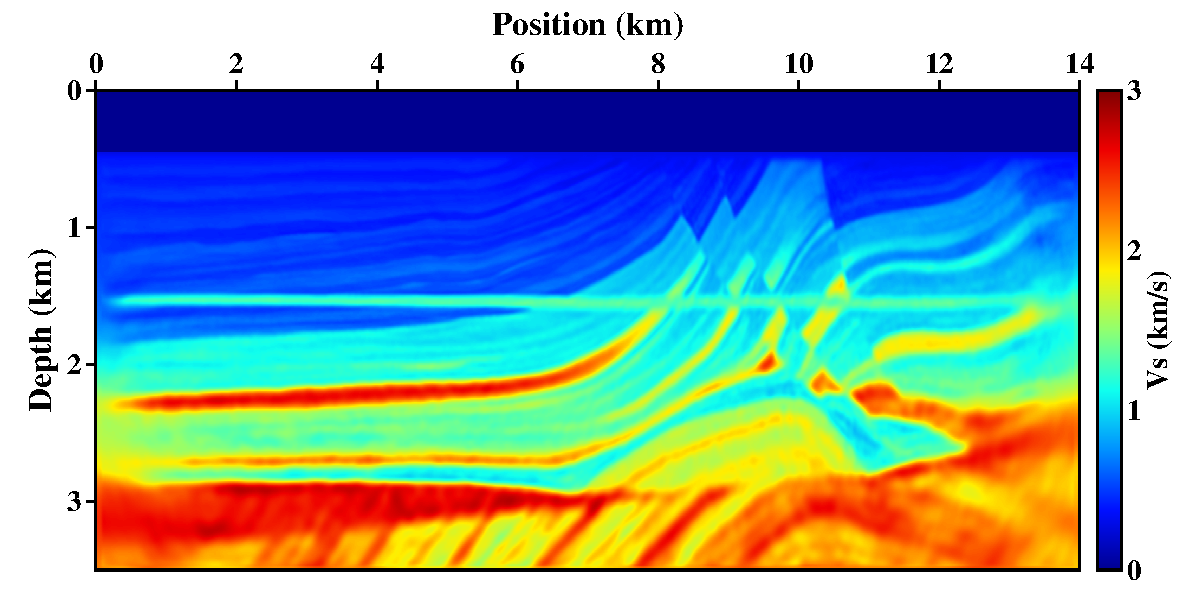
\includegraphics[width=7cm]{Figure/chapter02/tariqsugresult/Fig/devs.pdf}}
        \caption{
			反演的Marmousi-II模型:其中左侧为$V_p$,右侧为$V_s$. (a), (b)为PCG方法反演结果;(c), (d)为模式解耦方法反演结果。
%        The inverted Marmousi-II model: The inverted results using the PCG (a, b)
%            and the MD-based methods (c, d).
%        (a) and (c) are $V_p$ models while (b) and (d) are $V_s$ models.
    }
    \label{fig:MarInvert}
    \end{center}
\end{figure}
过去十年间,很多EFWI策略被用在了OBC地震数据中。在低频数据存在的情况下,重建低Poisson比的模型(硬海底)相对比较容易\cite[]{bae:2012}。
然而,软海底环境在现实中更为普遍。这种情况下,PS转换能量非常有限,同时反演中的非线性程度以及参数间的耦合也
会变得更加严重。为了应对这种更真实的软海底情况,
如图\ref{fig:MarInitTrue}(a)和(b)所示,我们用Marmousi-II模型中的原始P波与S波速度来测试我们的算法。不同参数间非一致的结构能更明显地表明参数间的耦合。
为了更好的展示MD方法的优势,我们在S波速度模型1.5km深处添加一个高速的薄层。在反演中,我们采用交错网格有限差分来计算正传与共轭波场,空间采样间隔为5m。
记录总时间为8s,时间采样间隔为0.5ms。共有40炮合成数据,炮点深度在20m的水深处,2800个检波点放置于海底来模拟OBC观测。初始模型通过SU软件中的smooth2函数
来平滑真实模型产生,平滑半径为300m。我们采用与前一实验同样的多尺度策略,但是每阶段最大迭代次数扩大为40次。

图\ref{fig:MarInvert}的结果证明了MD方法比常规方法能提供更好的反演结果。
在模型浅部(约1.5km),两种方法都能很好的恢复$V_p$模型,而常规方法恢复的$V_s$模型
分辨率较低。常规方法中,S波速度模型中的高速异常薄层给反演造成了很大的挑战,如图\ref{fig:MarInvert}(a)和(b)中所示,反演结果受到了很强的参数耦合
的干扰,尤其是在左侧的高速异常薄层区域。这就导致了在该异常薄层下方构造的错位与不聚焦,如图中箭头所示。然而,模式解耦反演方法很好地避免了这些参数耦合效应,
获得了模型的许多细节,包括中部的断层与背斜构造。模型的纵向剖面(图\ref{fig:VertiProfile})
进一步证明了模式解耦反演方法获得了比常规方法更好的结果。
\begin{figure}[!htb]
	\begin{center}
		{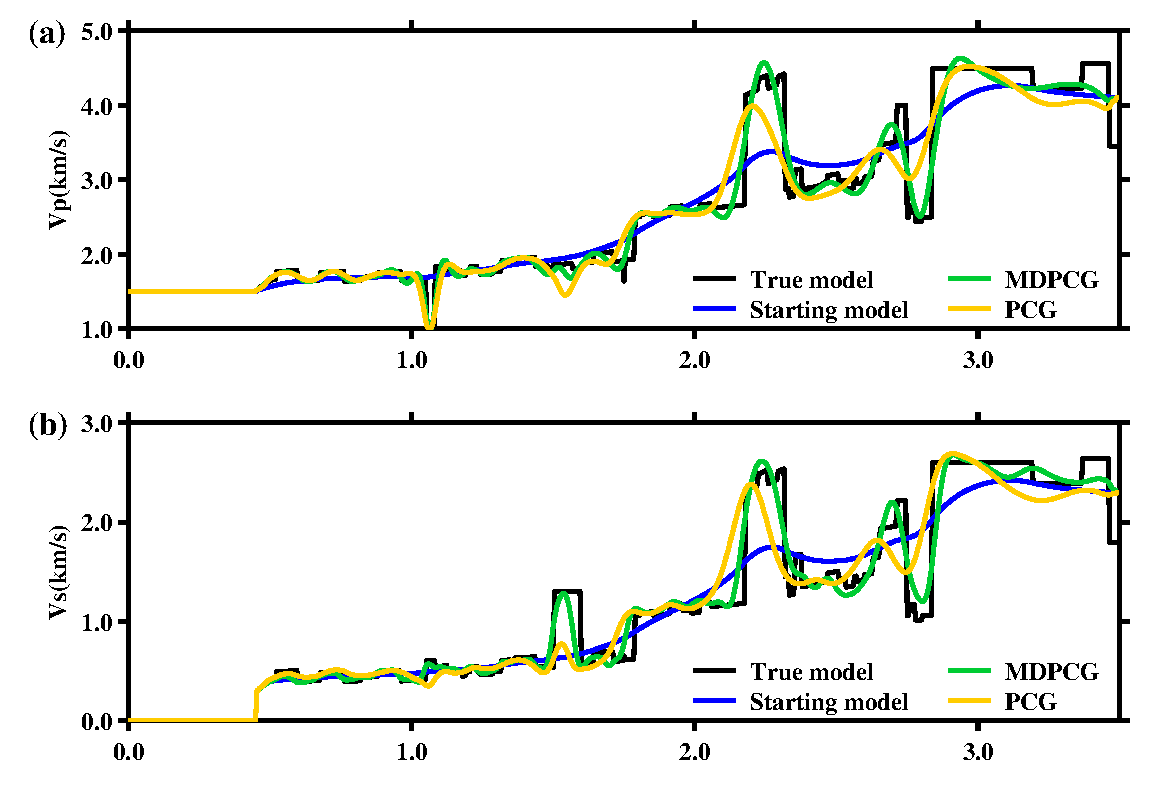
\includegraphics[width=10cm]{Figure/chapter02/tariqsugresult/Fig/new3km.pdf}}
		{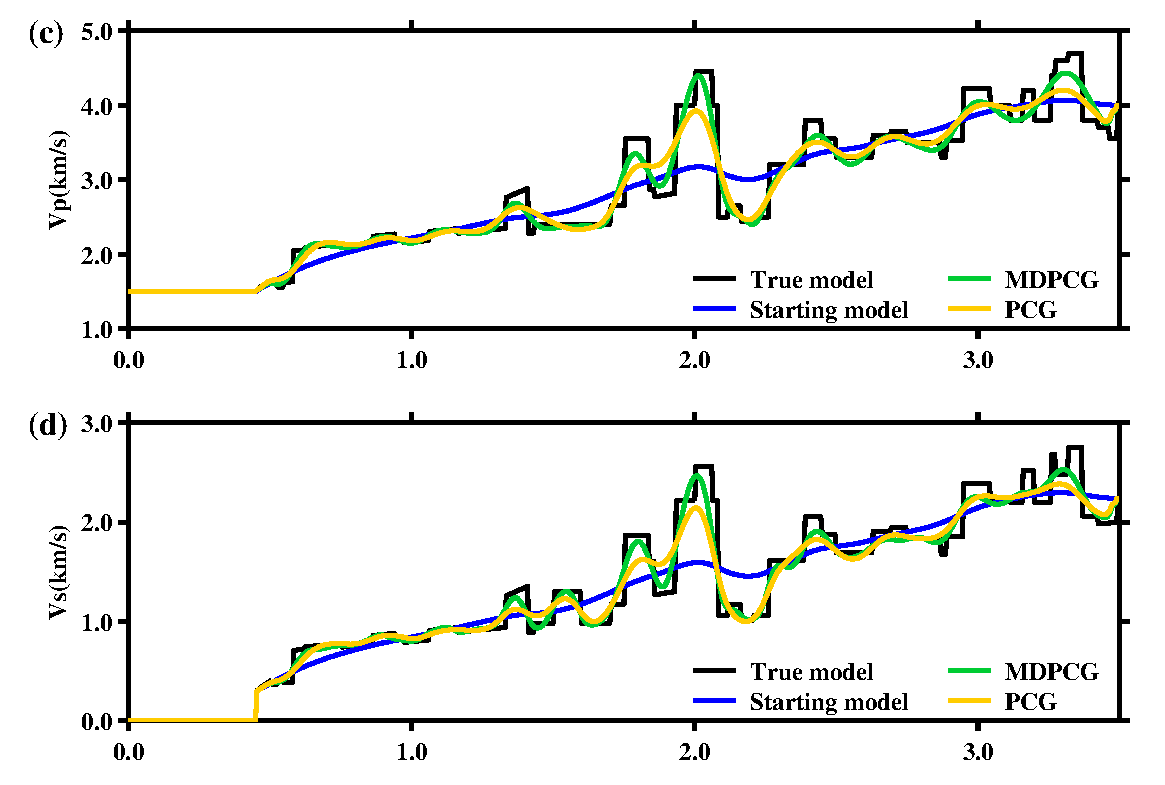
\includegraphics[width=10cm]{Figure/chapter02/tariqsugresult/Fig/new9km.pdf}}
		\caption{
		模型在3.0km(a,b)和9.0km(c,d)处的纵向剖面。黑线和蓝线分别代表真实和初始模型;黄线与绿线分别代表PCG和模式解耦方法反演结果。
%		The velocity profiles at 3.0 km (a, b) and 9.0 km (c, d) with the true models
%			(black),
%			the initial models (blue), the PCG-based (yellow) and MD-based (green)
%			inverted models.
	}
	\label{fig:VertiProfile}
	\end{center}
\end{figure}

\begin{figure}[!htb]
    \begin{center}
        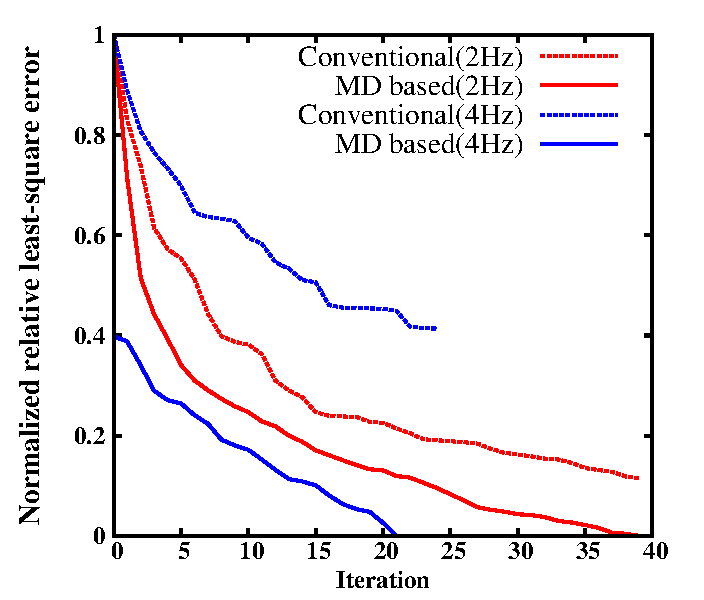
\includegraphics[width=10cm]{Figure/chapter02/tariqsugresult/Fig/L2.pdf}
        \caption{
			归一化后的L2残差随迭代次数的变化。红色与蓝色代表第一和第二阶段的反演,虚线代表PCG方法
			实线代表模式解耦方法。
%            Normalized L2 norms as a function of iteration for the PCG-based (dash)
%            and MD-based (solid) inversions in the first (red) and second (blue)
%            stages.
    }
    \label{fig:L2}
    \end{center}
\end{figure}
图\ref{fig:L2}展示了在前两个阶段的反演中,归一化的目标函数值随迭代次数的下降曲线。可以看到,模式解耦反演方法要比常规方法收敛更快。在第一个阶段,模式解耦
反演方法的数据拟合程度更高,同时获得了更准确的中低波数模型更新。在第二个阶段,常规梯度方法最终在25次迭代之后停止更新且数据残差相当大,而模式解耦反演方法
在22次迭代后数据残差快速下降达到终止条件。这些结果说明利用模式解耦对梯度做预条件可以很有效地在反演中降低参数耦合从而加速收敛。
\begin{table}[!htb]
    \caption{The total computational costs}
    \label{table:TotalComputime}
	\centering 
%   \begin{tabular}{|c|c|c|c|c|c|c|}
%   \begin{tabular}{|p{1.8cm}|c|c|c|c|p{2.2cm}p{2.3cm}p{2cm}|}
    \begin{tabular}{p{1.8cm}p{1.0cm}p{1.0cm}p{1.0cm}p{1.2cm}p{1.0cm}p{1.0cm}}
%    \begin{tabular}{|p{1.8cm}|p{1.0cm}p{1.0cm}p{1.0cm}p{1.2cm}|p{1.0cm}p{1.0cm}|}
    \hline
    \quad&\multicolumn{4}{c}{Iteration number}&\multicolumn{2}{c}{Time spent (hour)} \\
%   \quad&\multicolumn{4}{|c|}{Iteration number}&\multicolumn{2}{|c|}{Computing Time (hour)} \\
    \hline
%   Method & stage1 0-2Hz &stage2 0-4Hz&stage3 0-6Hz&stage4 0-10Hz&Total &Average \\
    \multirow{2}{*}{Method} & stage1 &stage2 &stage3 &stage4 &\multirow{2}{*}{Total}
    &\multirow{2}{*}{Average} \\
    & 0-2Hz &0-4Hz&0-6Hz&0-10Hz\\
    \hline
    Conventional&  40   &25&5& 7  &41.4&0.538\\
    MD-based &   40  & 22 &33 &13&68.3&0.632\\
    \hline
    \end{tabular}
\end{table}

表\ref{table:TotalComputime}
中列出了在8节点(每节点15核)的工作站上每个阶段的迭代次数和总的计算时间。每个阶段我们设定最大迭代次数为40次。因为当搜索不到合适步长的时候迭代会自动终止,所以
不同阶段的实际迭代次数并不相同。在常规方法中,严重的参数耦合效应会影响从低频数据中重建出合适的宏观模型,这就导致在高频阶段无法获得合理的梯度方向,使得迭代过早终止。而模式解耦方法可以一定程度回避参数耦合,因此其在低频阶段能够重建出合适的宏观模型,从而使得高频阶段的梯度更合理,迭代次数更多。这也是为什么模式解耦方法能
获得更准确,分辨率更高的反演结果。总的来说,模式解耦方法需要更多的迭代次数,也因此计算时间更多。但是每次迭代的平均用时只增加了18\%左右。
\section{讨论}
\subsection{更进一步分解梯度的必要性}
我们可以对正传与反传波场分别解耦从而获得对应不同模式转换的解耦梯度,也即PP、PS、SP和SS。但是,很难设计出一个单独使用某一模式转换数据的EFWI策略,因为我们无法
采用P/S分离的算法在观测面上区分入射波场的类型,也即无法区分PP与SP(或PS与SS)。否则,只能使用分解后的单模式地震数据来进行单参数反演。例如
Ren和Liu\cite{ren.liu:2016},在其四步反演策略的第二步中,当有很强的S波能量时,只采用分解的P波场来反演P波速度,或者在弱S波能量时仅仅拟合S波数据来反演S波速度。


需要注意的是,在梯度计算中分解正传波场等价于次级源(或背景波场)的波模式,而次级源是Frech{$\acute{e}$}t导数中的一部分。因此我们可以将该线性问题写为:
\begin{equation}
    \mathbf{J}^{XY}\delta\mathbf{m}=\mathbf{\delta u}^{XY},
    \label{eq:JXY}
\end{equation}
其中$X$和$Y$分别表示次级源与散射Green's函数的波模式,$\mathbf{\delta u}^{XY}$则表示${X}$-to-${Y}$模式的扰动波场。根据方程\eqref{eq:ResoOperP}的推导方式,我们
可以获得相应的分辨率矩阵:
\begin{equation}
    \mathbf{R}^{XY}=\mathbf{H}_a^{-g}\mathbf{J}^{\dagger}\mathbf{J}^{XY}. 
    \label{eq:RXY}  
\end{equation}
图\ref{fig:ResoMN}展示了PP、PS、SP和SS模式的分辨率矩阵,其观测系统与图\ref{fig:Resolution}中一致,但是采用了P和S的混合震源。图中的带对角结果是由于更加复杂的
波现象。可以看到,$\mathbf{R}^{PP}$ 与$\mathbf{R}^P$十分类似,而$\mathbf{R}^{SP}$却几乎为空矩阵。这表明用PP波数据来反演$V_p$会受到来自$V_s$的干扰。而SP波数据
则对两个参数的反演都贡献很小。从Ren和Liu\cite{ren.liu:2016}的例子中(见其文中图19与20),即使震源中含有足够强的S波能量,SP梯度也是很弱且有很多噪音。一个
可能的解释就是如图\ref{fig:SPSS}所示,S-to-P的散射能量很弱。此外,我们也难
区分出PS和SS模式的贡献,因为从图\ref{fig:ResoMN}中看到,$\mathbf{R}^{PS}$和
$\mathbf{R}^{SS}$的非零元素分布非常一致。因此,想通过分解正传波来对进一步地降低参数耦合效应的潜力非常有限,尽管这样会带来更多的计算量。这也是为什么我们只
分解反传波场来对梯度进行预条件。
\begin{figure}[!htb]
    \begin{center}
        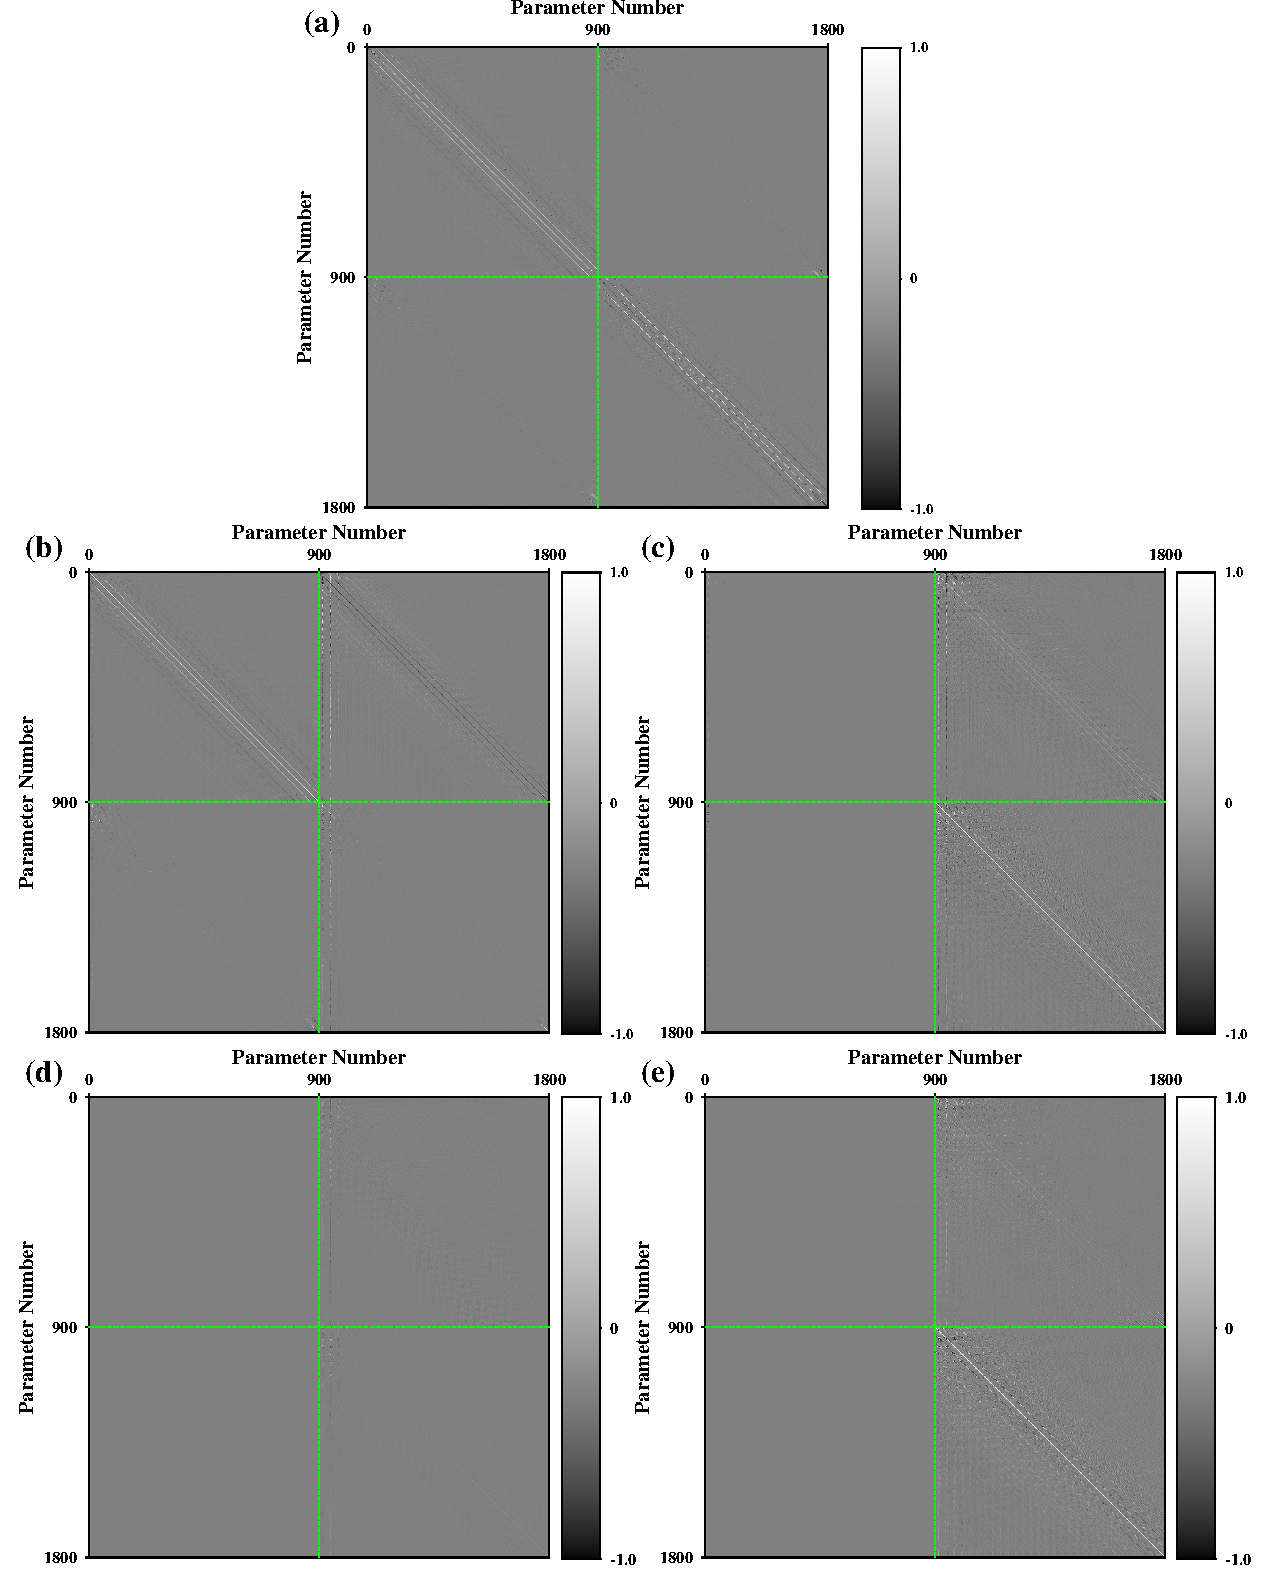
\includegraphics[width=12cm]{Figure/chapter02/ResoOpera/Fig/resolutionMN.pdf}
        \caption{
			采用混合震源时不同模式数据转换的分辨率矩阵。
%            Resolution matrices associated with different mode conversion data using
%            mix-source:
            (a) $\mathbf{R}$, (b) $\mathbf{R}^{PP}$, (c) $\mathbf{R}^{PS}$, (d)
            $\mathbf{R}^{SP}$ 和(e)
            $\mathbf{R}^{SS}$.
    }
    \label{fig:ResoMN}
    \end{center}
\end{figure}

\begin{figure}[!htb]
    \begin{center}
        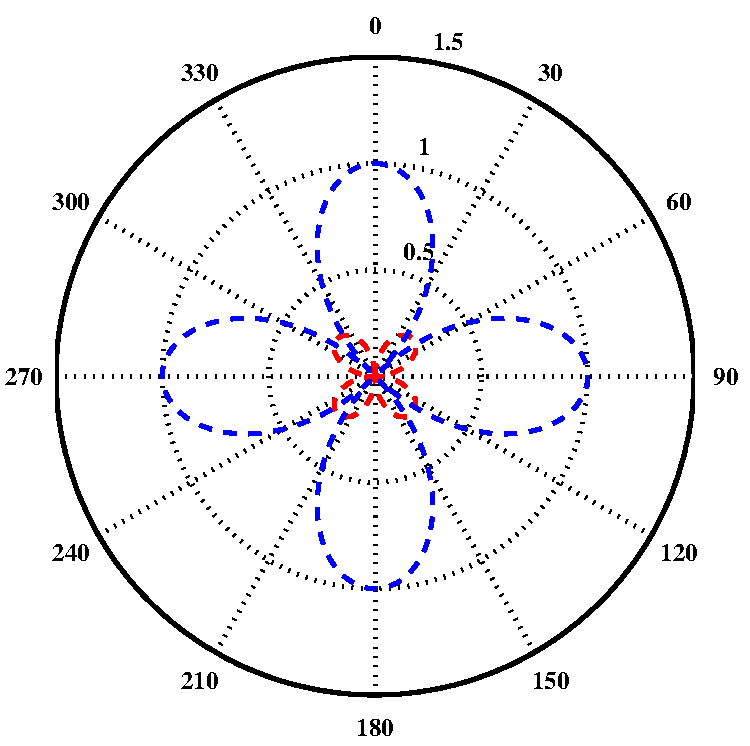
\includegraphics[width=5cm]{Figure/chapter02/radiationpattern/Fig/SPSS.pdf}
        \caption{
			归一化的SP模式(红色)和SS模式(蓝色)的辐射模式。
%            Radiation pattern of SP and SS modes with a same normalization: SP
%            mode (red) and SS mode (blue).
    }
    \label{fig:SPSS}
    \end{center}
\end{figure}
\subsection{密度模型的反演}
密度扰动同时散射P-和S-波,但是却几乎不影响两种波模式的相位或者走时。这种模式的散射能量大多与入射波场的传播方向相反\cite[]{wu.aki:1985,tarantola:1986}。因此,
密度作为一个次级效应的参数,由于其微弱的敏感性和多参数的耦合效应\cite[]{tarantola:1986,forgues.lambare:1997},其很难被重构。这也是为何很多EFWI的研究只考虑
常密度的情形\cite[]{shipp:2002,sears2008,brossier2009}。只有很少一部分的工作能够从多尺度策略和(或)不同参数化方式的选取中获得较为合理的密度反演结果
\cite{jeong2012full}。最近,基于子空间的方式\cite[]{kennett:1988},Xu和McMechan\cite{xu.mcmechan:2014}提出了一种多步长的梯度类方法来压制$V_p$, $V_s$和
$\rho$之间的串扰。Yang等\cite{Yang:2016}采用改进的散射积分法(SI)来通过Hessian的逆来提高声波FWI中$V_p$和$\rho$的估计。尽管Ren和Liu\cite{ren.liu:2016}提出了
基于波场解耦的四阶段多尺度策略来做EFWI,但是他们只是在第二阶段中采用了P/S分离来压制$V_p$和$V_s$之间的耦合,然后通过多步长的手段来改善三参数同时反演的结果。
在他们展示的overthrust模型中,密度的反演结果仍然偏离真实模型较远。因此非常有必要进一步调查模式解耦预条件方法对改善密度反演的潜力。
\begin{figure*}
    \begin{center}
        \subfloat[]{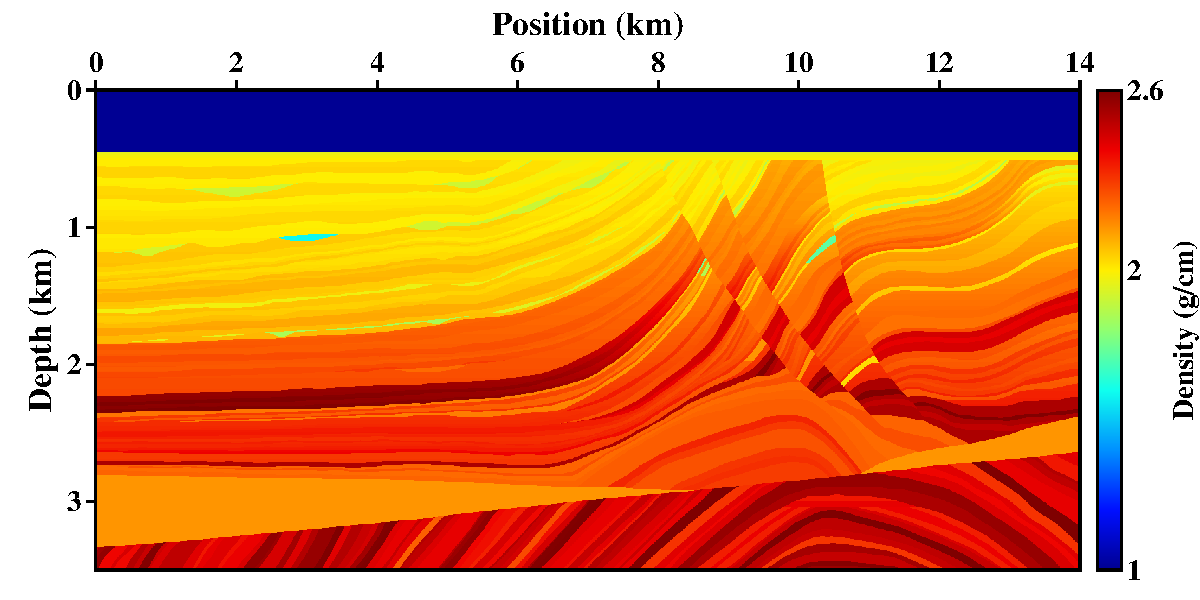
\includegraphics[width=7cm]{Figure/chapter02/tariqsugresult/Fig/truerho.pdf}}
        \subfloat[]{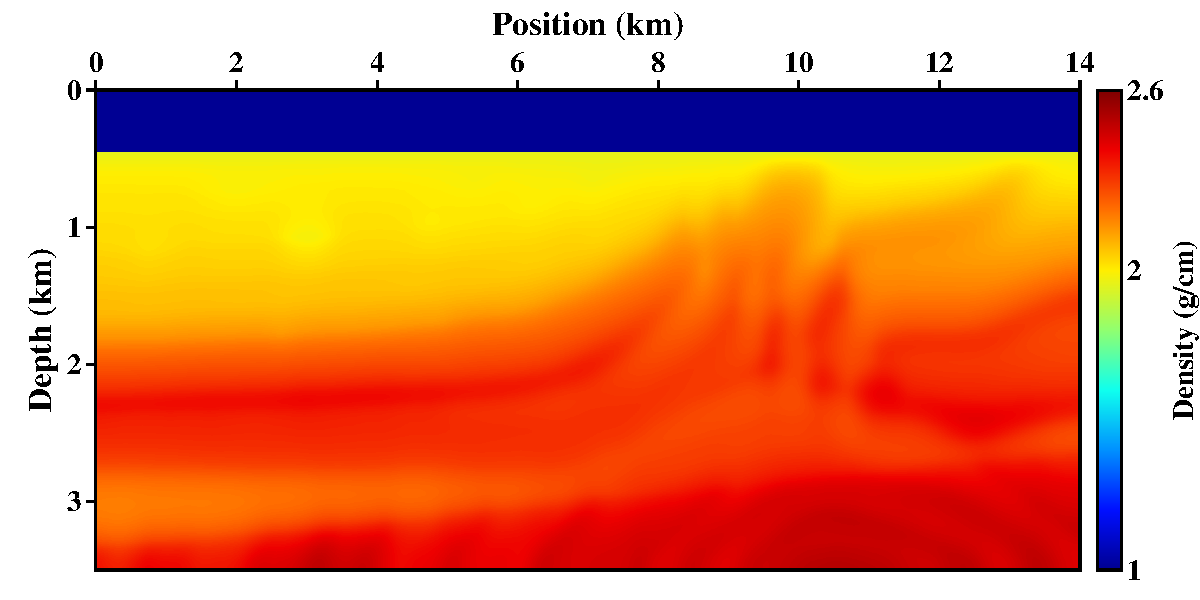
\includegraphics[width=7cm]{Figure/chapter02/tariqsugresult/Fig/initrho.pdf}}
    \caption{
		真实(a)和初始(b)Marmousi-II的密度模型
%                The true (a) and initial (b) density Marmousi-II model.
    }
    \label{fig:Marrho}
    \end{center}
\end{figure*}

采用速度-密度参数化方式,密度的梯度公式可以表示为\cite[]{mora:1987,kohn:2012}:
\begin{equation} 
    \hat{\mathbf{g}}_{\rho}=(V^2_p-2V^2_s)\mathbf{g}_{\lambda}+V^2_s\mathbf{g}_{\mu}+\mathbf{g}_{\rho},
    \label{eq:Gradient_rho} 
\end{equation}
其中$\mathbf{g}_{\lambda}$, $\mathbf{g}_{\mu}$和$\mathbf{g}_{\rho}$为采用$\rho$-Lame参数化时的梯度,也即:
    \begin{equation} 
        \begin{split}
                \mathbf{g}_{\lambda}&=-\int_{0}^{T}\frac{\partial u_i}{\partial
        x_j}\frac{\partial \psi_k}{\partial x_l}
        \delta_{ij}\delta_{kl}dt,\\
                \mathbf{g}_{\mu}&=-\int_{0}^{T}\frac{\partial u_i}{\partial
        x_j}\frac{\partial \psi_k}{\partial x_l} 
        (\delta_{ik}\delta_{jl}+\delta_{il}\delta_{jk})dt,\\
                \mathbf{g}_{\rho}&=-\int_{0}^{T}\frac{\partial^2 u_i}{\partial
        t^2}\psi_idt.
        \end{split}
        \label{eq:DeGradient_vpvsrho}
    \end{equation}
前文所述中,在Born近似下,S波数据对$V_s$的扰动更加敏感,基于以上考虑我们采用了解耦梯度的方式来同时反演$V_p$和$V_s$。然而考虑密度反演时,由于密度扰动
同时产生S-与P波散射数据,因此上述逻辑就不再成立。我们联合方程\ref{eq:DeGradient_vpvs}和\ref{eq:Gradient_rho}来进行三参数同时反演。我们采用同样的
观测系统和反演策略并引入原始Marmousi密度模型来进行数值实验。

如图\ref{fig:InvertWithRho}所示,由于强烈的参数耦合效应,采用PCG优化的常规EFWI对三个参数都未能获得合理的重建。在模型左侧软海底较厚的区域,在引入密度变化后,
反演的病态性变得更加剧烈。$V_p$和$V_s$之间的耦合甚至导致反演结果中结构的错位。在采用模式解耦预条件后, $V_p$和$V_s$的反演都获得了很大的改善,但是密度的反演
结果仍然不准确,并包含了较多来自$V_s$扰动的“脚印”。不管如何,我们可以看到模式解耦可以降低反问题病态程度并提高反演模型的分辨率。但是若想改善密度反演结果,
就需要用到更多的多尺度策略以及Hessian的逆的信息来更好的压制参数耦合效应。
\begin{figure*}
    \begin{center}
        \subfloat[]{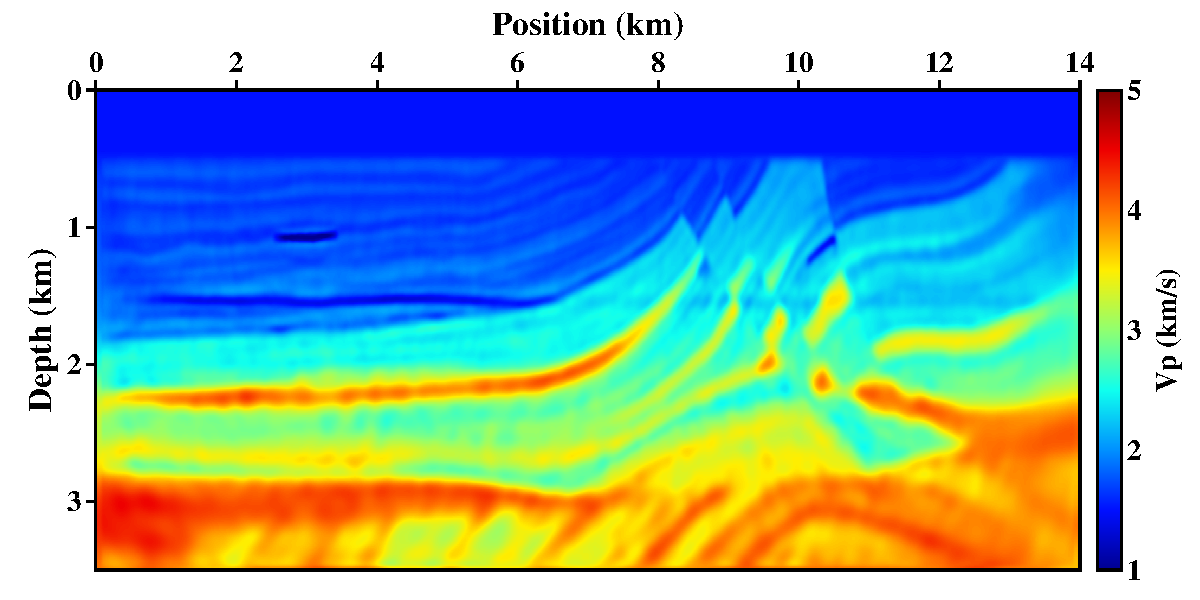
\includegraphics[width=7cm]{Figure/chapter02/tariqsugresult/Fig/1nodevp.pdf}}
        \subfloat[]{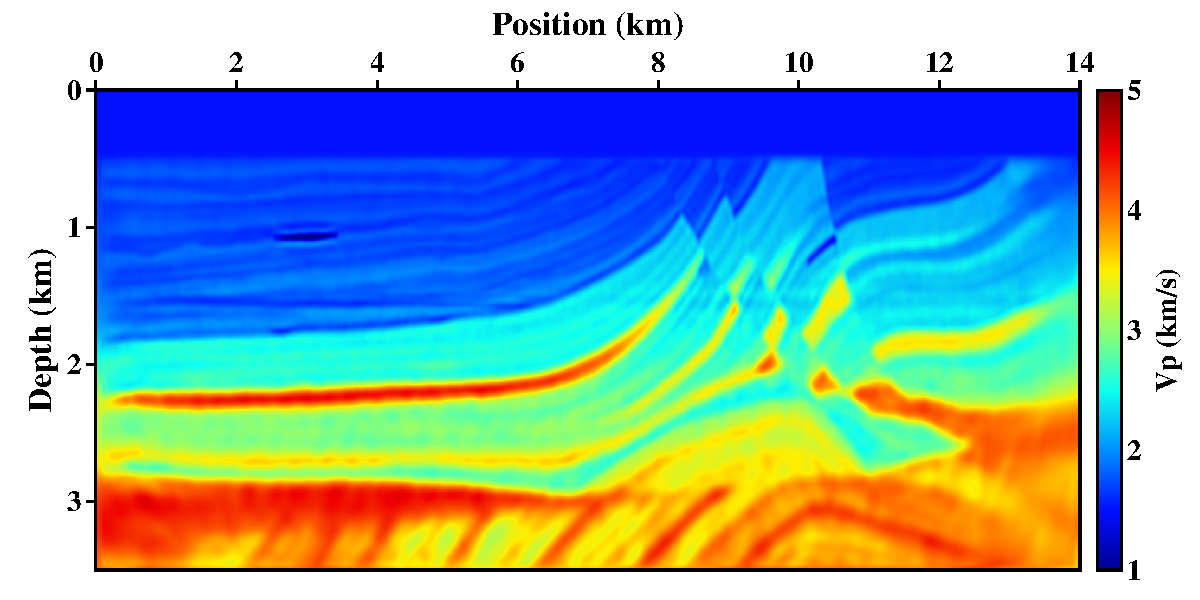
\includegraphics[width=7cm]{Figure/chapter02/tariqsugresult/Fig/1devp.pdf}}\\
        \subfloat[]{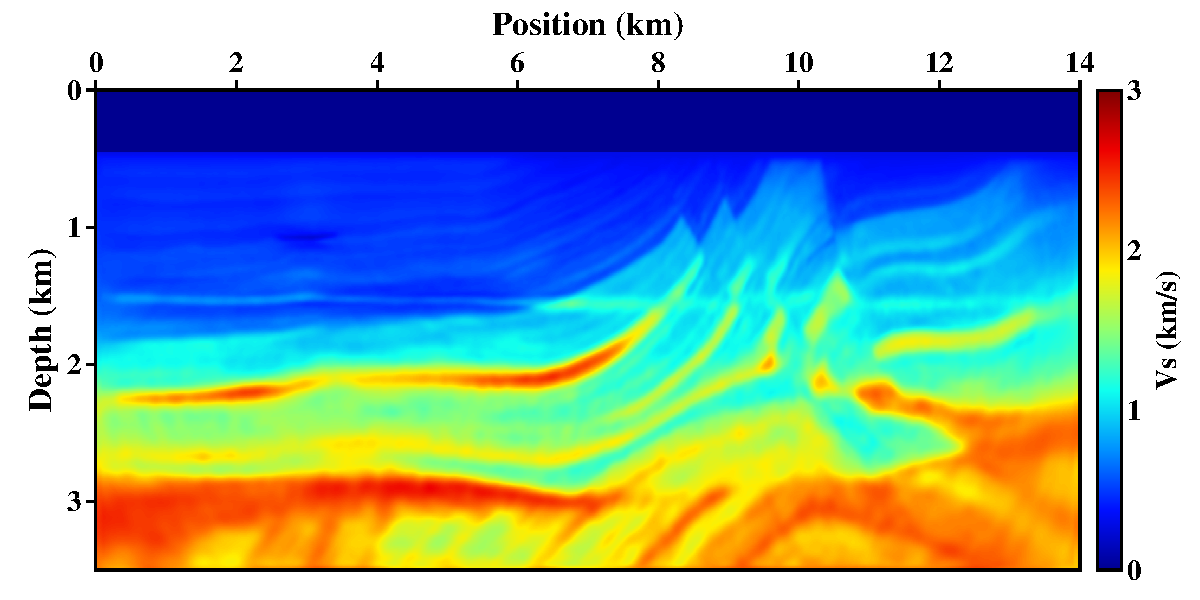
\includegraphics[width=7cm]{Figure/chapter02/tariqsugresult/Fig/1nodevs.pdf}}
        \subfloat[]{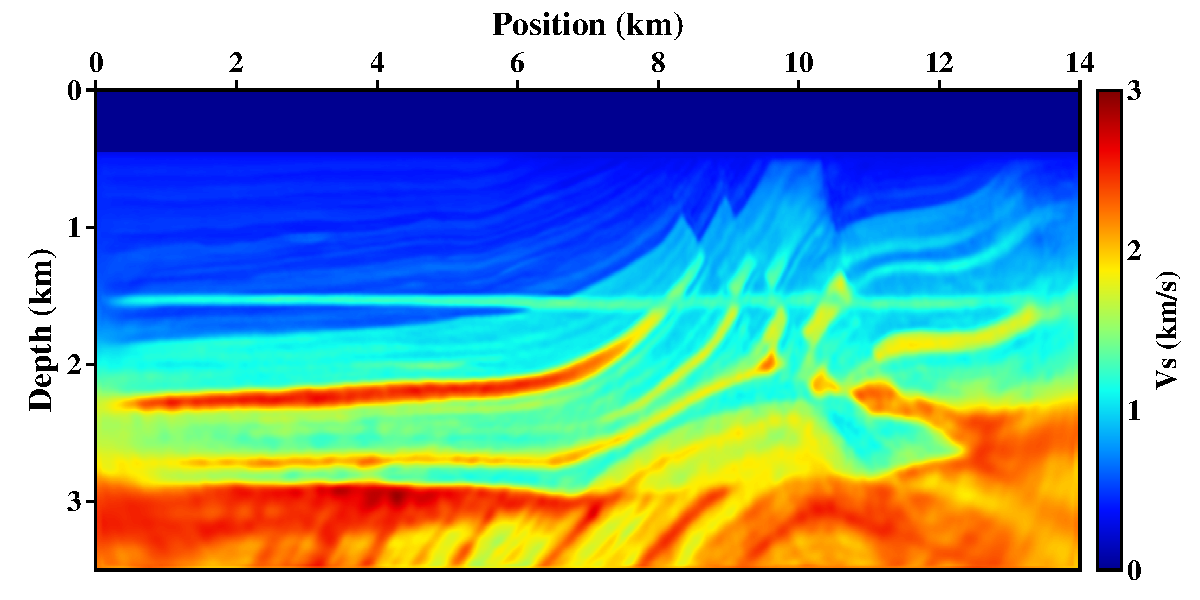
\includegraphics[width=7cm]{Figure/chapter02/tariqsugresult/Fig/1devs.pdf}}\\
        \subfloat[]{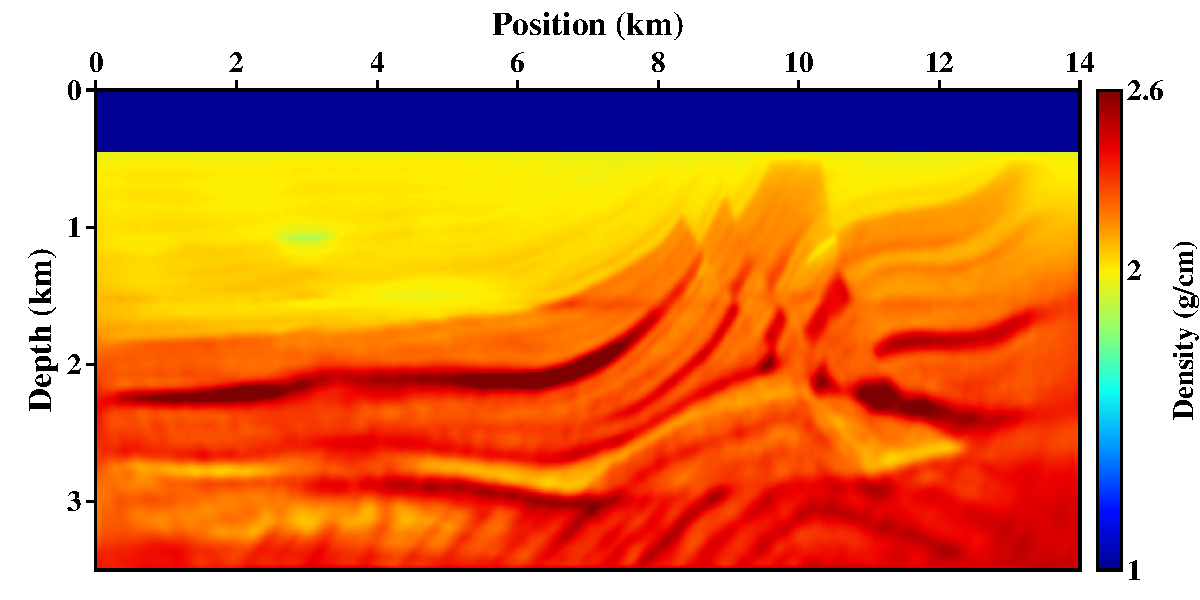
\includegraphics[width=7cm]{Figure/chapter02/tariqsugresult/Fig/1noderho.pdf}}
        \subfloat[]{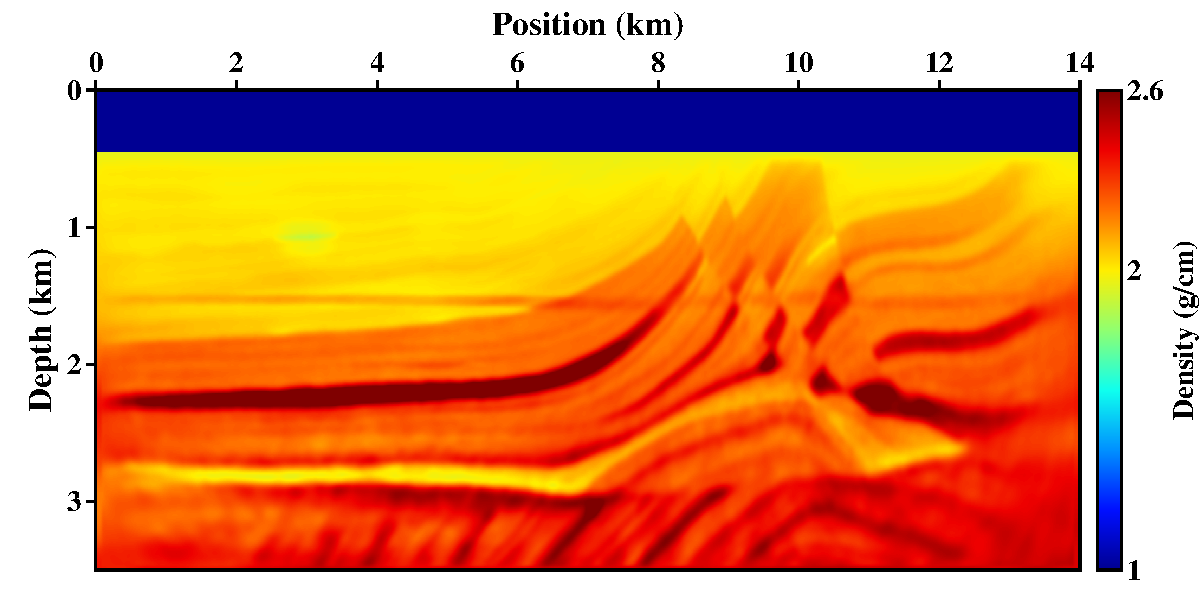
\includegraphics[width=7cm]{Figure/chapter02/tariqsugresult/Fig/1derho.pdf}}
        \caption{
			密度变化时常规和模式解耦的EFWI结果对比。左侧为常规PCG方法反演结果,右侧为模式解耦方法反演结果。
			其中(a),(b)为$V_p$; (c), (d)为$V_s$; (e), (f)为$\rho$。
%			Comparison between conventional and MD-based method with density
%            variation: (a) - (c) are the inverted $V_p$, $V_s$ and $\rho$ with
%            conventional method, (d) - (f) are the inverted $V_p$, $V_s$ and $\rho$
%            with MD-based method. 
		}
    \label{fig:InvertWithRho}
    \end{center}
\end{figure*} 
\begin{figure*}
    \begin{center}
        {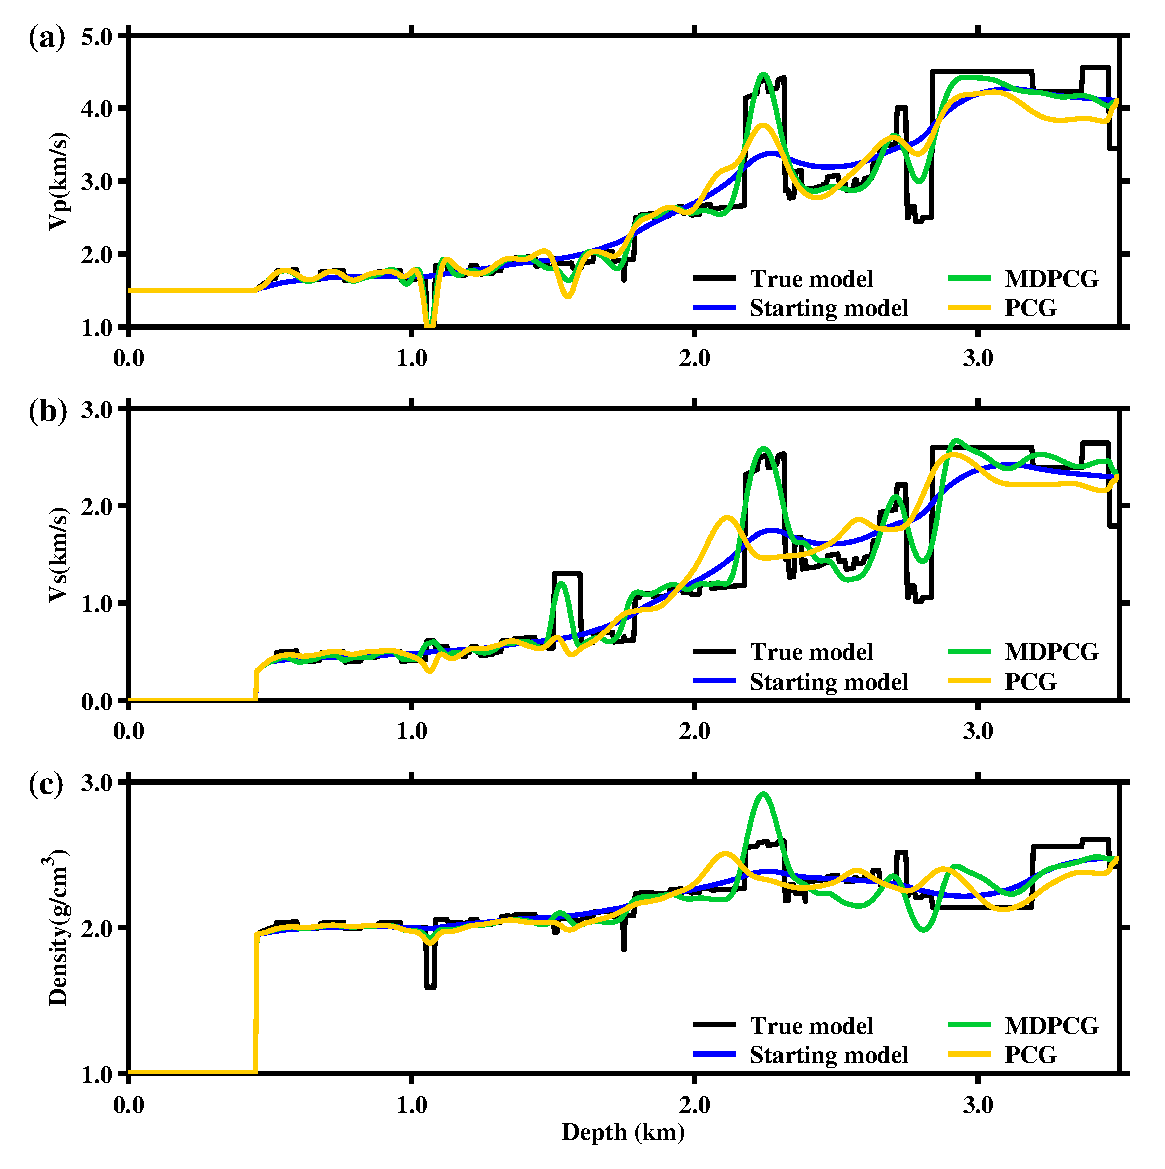
\includegraphics[width=10cm]{Figure/chapter02/tariqsugresult/Fig/3kmrho.pdf}}
        \caption{
			速度与密度模型在3.0km处的纵向剖面。
			黑线和蓝线分别代表真实和初始模型;黄线与绿线分别代表PCG和模式解耦方法反演结果。
%        The velocity and density profiles at 3.0 km (a, b)  with the true models
%            (black),
%            the initial models (blue), the PCG-based (yellow) and MD-based (green)
%            inverted models.
    }
    \label{fig:RhoProfile3km}
    \end{center}
\end{figure*}
\begin{figure*}
    \begin{center}
        {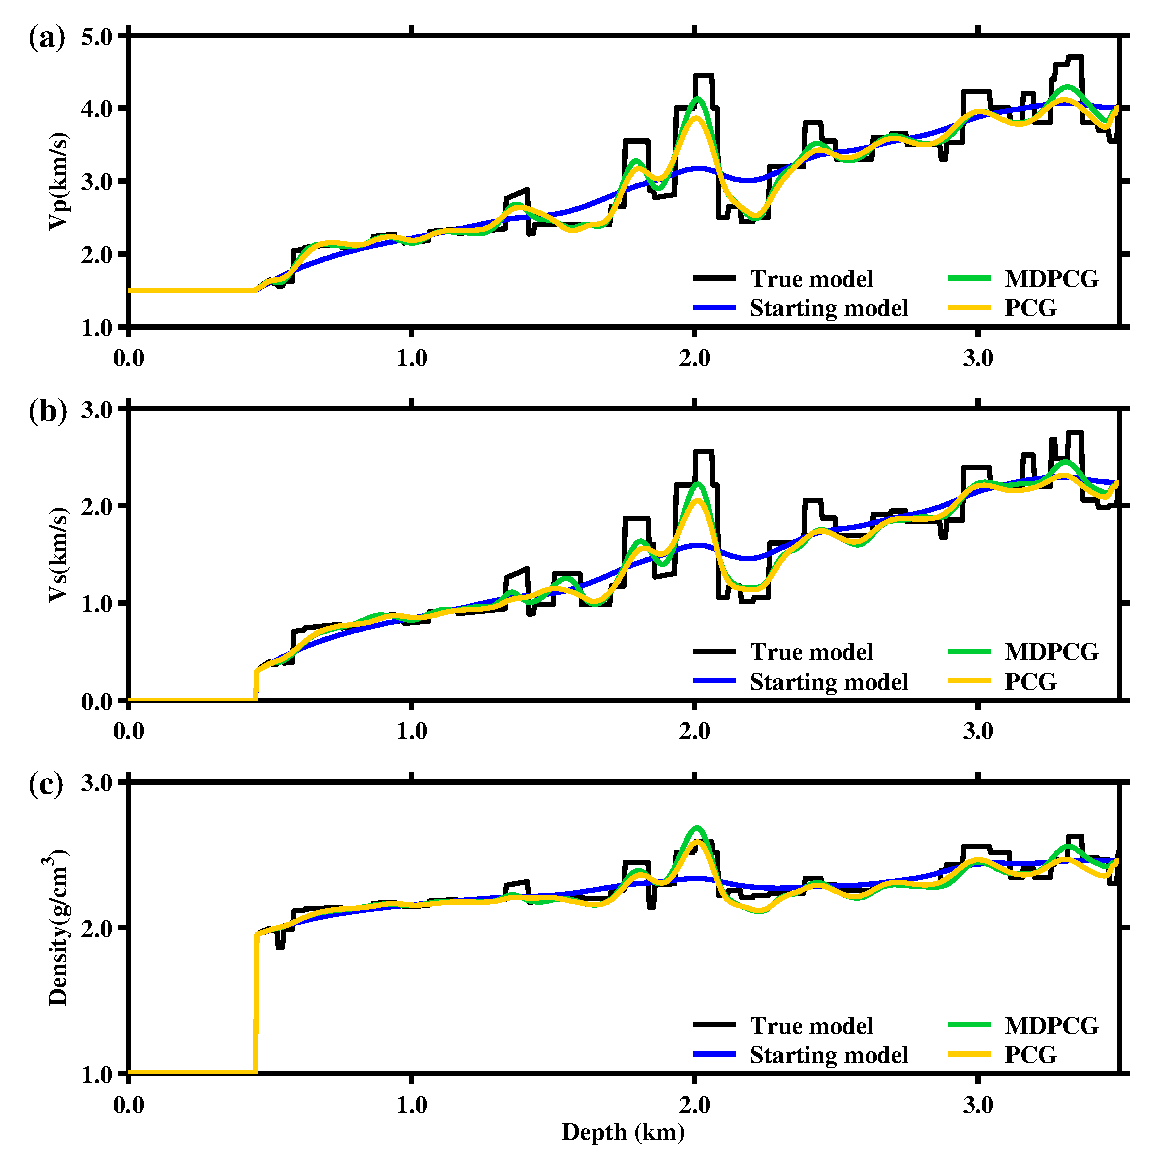
\includegraphics[width=10cm]{Figure/chapter02/tariqsugresult/Fig/9kmrho.pdf}}
        \caption{
			速度与密度模型在9.0km处的纵向剖面。
			黑线和蓝线分别代表真实和初始模型;黄线与绿线分别代表PCG和模式解耦方法反演结果。
%        The velocity and density profiles at 9.0 km (a, b)  with the true models
%            (black),
%            the initial models (blue), the PCG-based (yellow) and MD-based (green)
%            inverted models.
    }
    \label{fig:RhoProfile9km}
    \end{center}
\end{figure*} 

\section{本章小结}
多参数反演的耦合效应使得常规梯度方法EFWI受到很大挑战,即使是只考虑P-和S波速度的反演。辐射模式表明速度扰动都会产生P波数据扰动从而导致在特定散射角范围内的
串扰效应。相反,S波扰动波场则只与S波速度扰动相关。通过引入弹性波模式解耦,我们发现在解耦之后,不同波模式的Frech{$\acute{e}$}t和数据残差之间的互相关对梯度
的贡献非常微弱。通过该交叉项近似,我们导出了基于模式解耦的梯度,该梯度可以通过伴随状态法快速计算得到。采用解耦之后的Frech{$\acute{e}$}t导数,我们调查了
Hessian以及分辨率矩阵对应于P波与S波数据的相关分量。这些调查结果确认了在S波速度的梯度计算中分离P波分量可以降低参数耦合的效应。由此,采用基于模式解耦的方法
来反演$V_s$等价于采用S波数据的单参数反演。如果能找到较好的预条件算子来消除S波数据的照明以及有限带宽效应,则该方式总能获得近似GN方法的收敛速度而不涉及
任何Hessian相关的计算。而对于双参数同时反演,$V_s$反演的改善可以明显提高$V_p$的反演结果。数值实验,尤其是包含软海底结构的Marmousi模型,证明了模式解耦方法
对降低参数耦合、加速收敛的有效性。

目前为止,通过波形反演来重建可靠的密度结果仍然非常困难。正如我们所看到,模式解耦并未能改善密度反演结果。但是在引入密度扰动,反演病态性明显剧增后仍能保证
获得合理的$V_p$和$V_s$结果。
